% Two-column extended manuscript ("left part / right part" journal layout).
% Self-contained: requires only article, tikz, natbib, booktabs.
% Compile: pdflatex main_twocolumn.tex  (run twice)
\documentclass[10pt,twocolumn]{article}
\usepackage[margin=0.72in,columnsep=0.24in]{geometry}
\usepackage{amsmath,amssymb,amsthm}
\usepackage{booktabs,multirow,array}
\usepackage{graphicx}
\usepackage{xcolor}
\usepackage{tikz}
\usetikzlibrary{shapes.geometric,arrows.meta,positioning,calc,fit,backgrounds,decorations.pathmorphing}
\usepackage[colorlinks=true,linkcolor=blue!55!black,citecolor=blue!55!black,urlcolor=blue!55!black,
            pdftitle={Priced Memory Allocation with Exact Trace Valuation: A Study on Linear Predictors},
            pdfauthor={Hazem Mohamed Ali Hassan},
            pdfsubject={Memory hierarchy structure as the solution of a priced allocation problem},
            pdfkeywords={memory allocation, continual learning, caching, routing, leave-one-out valuation}]{hyperref}
\usepackage[numbers,sort&compress]{natbib}
\usepackage[T1]{fontenc}
\usepackage{lmodern}
\usepackage{microtype}

\linespread{0.965}\selectfont
\setlength{\parskip}{0pt}
\newtheorem{theorem}{Theorem}
\newtheorem{lemma}{Lemma}
\newtheorem{proposition}{Proposition}
\newtheorem{corollary}{Corollary}
\newtheorem{assumption}{Assumption}
\theoremstyle{definition}
\newtheorem{instance}{Numerical instance}
\newcommand{\PES}{PES}
\DeclareMathOperator{\argmax}{arg\,max}
\DeclareMathOperator{\argmin}{arg\,min}

\title{Priced Memory Allocation with Exact Trace Valuation:\\[4pt]
\large A Study on Linear Predictors}
\author{Hazem Mohamed Ali Hassan\\\small sim.HazemMohamed81084@alexu.edu.eg}
\date{}

\begin{document}
\twocolumn[
\begin{@twocolumnfalse}
\maketitle
\begin{abstract}
Learning systems hard-code where knowledge lives: activations are ephemeral, optimizer state is scratch,
and parameters are permanent. We replace this inherited partition with an allocation problem. A learner
maintains many traces of information and a small set of stores with different persistence
profiles---maintenance tariff, decay rate, capacity---and pays explicit prices for keeping and for moving
information. The resulting rule, \emph{Persistence-Economics Selection} (\PES), places each trace where its
accumulated responsibility for prediction error best covers its costs. The theory here is exact rather than
heuristic: we prove a \emph{closed-form solution} of the static
allocation problem---sort cross-store margins, route negative-margin traces to slow storage, clip the fast
occupancy count to the capacity interval---with a complete exchange proof and a uniqueness corollary for the
eviction rule; per-window optimality of the fee-gated max--min exchange rule against adversarial value
sequences; an unconditional throughput ceiling for hysteresis-controlled routing; and a constructive
corner-pricing theorem recovering six established mechanisms (exact caching, weight decay, EWC/SI
protection, delta-rule decay, scheduled consolidation, learned single-store eviction) as boundary points of
one objective. Two impossibility results with fully verified numerical instances quantify where optimality
necessarily ends: synergistic valuation breaks additive-slotting optimality by an explicit $17.6\%$ gap of
optimal value --- one point of a family whose shortfall is unbounded --- and
migration budgets admit unbounded look-ahead advantages that connect directly to the measured dose--response
law. A second theory layer makes the guarantees tight: the deployed fee-gated margin rule is provably
\emph{unboundedly} non-competitive against a dynamic oracle, while its accumulating variant is exactly
$2$-competitive (matching the deterministic ski-rental lower bound); independent slotting is exact exactly
on modular value; honest deletion pricing under rare interactions requires $\Theta(1/p_{\mathrm{co}})$
stream samples (Le Cam), proving the observed density--exactness tradeoff fundamental; and the
migration--quality frontier is linear with an explicitly pinned slope. Empirically, replacing a cheap gradient-magnitude price with an exact leave-one-out loss price halves
retention error ($p=0.002$), erasing a significant deficit to fixed-schedule consolidation with every other
mechanism held fixed---routing quality tracks \emph{price quality}, not routing structure. Routing
throughput obeys a dose--response law in transition costs spanning $175\times$, while maintenance tariffs
never bind at tested scales: the operative price of memory is movement, not storage. Under genuinely scarce
memory---routing state far smaller than the input dimension---the unlimited-memory ceiling collapses:
unconstrained dense {SGD} falls from best to worst under drift, significantly behind priced routing
($p{=}0.021$, $n{=}10$). Failed pre-registered predictions are reported with diagnoses. We close by mapping the framework onto five deployment
domains---LLM {KV}-cache management, on-device continual learning, agent memory pipelines, tiered storage
systems, and synaptic consolidation---specifying for each what plays the role of trace, store, tariff, and
fee, and deriving falsifiable predictions per domain. The {KV}-cache proposal has since been empirically
tested on real transformer language models: the exact allocation rule delivers large, significant wins at
adequate capacity and fails at intermediate capacity exactly as the nonlinear-credit-assignment analysis
predicts, confirming both the predicted benefit and the predicted \S\ref{sec:nnport} failure mode on a
real system (\S\ref{sec:kvval}).

\medskip
\noindent\textbf{AI use disclosure.} AI tools were used for code development assistance and manuscript
review only. All experimental design, execution, and analysis were conducted by the author under
pre-registered protocols; the author takes full responsibility for the work.
\end{abstract}
\vspace{3mm}
\end{@twocolumnfalse}
]
\section{Introduction}\label{sec:intro}

Every deployed learning system embodies a decision it never made. Information sits in activations that die
at layer exit, in optimizer state erased at deployment, and in parameters that outlive everything else. The
timescale over which a fact persists follows from where it happens to sit, and where it sits was fixed
before training began. Other information disciplines solved this problem long ago. Library science moves a
volume from reading room to stacks to deep archive according to measured circulation; operating systems page
between {RAM} and disk by access frequency and recency; database engines migrate records between buffer pool
and cold storage by measured hit rates. In every mature case the defining property is the same: objects are
moved \emph{between tiers} according to measured value, movement is taxed, retention is earned rather than
granted, and the tier structure itself is justified by an explicit cost model. Machine learning rarely does
this. Its nearest analogues---two-speed synapses, surprise-gated memories, learned eviction---price one
commodity each (usually recency or surprise) inside a single store and leave the rest of the economy
unspecified.

Prior work loosens specific instances of the hard-coded partition. Fast weights~\citep{hinton1987fast,
ba2016using} introduce a second, rapidly decaying parameter set. Test-time training~\citep{sun2024testtime}
makes the hidden state a model that learns during inference. Titans~\citep{behrouz2024titans} writes to a
neural memory gated by surprise, and Nested Learning~\citep{behrouz2025nested} interprets optimizers as
associative memories arranged in nested optimization problems. In each case a decisive element remains fixed
by hand: the decay rate, the consolidation schedule, the level structure. The learner does not decide how
long things last; it inherits that.

This paper withdraws the inheritance. We provide a learner with many traces of information and a small set
of stores, each characterized by persistence economics: a maintenance tariff per step, an unattended decay
rate, and a capacity. Moving a trace between stores costs a fee. One question organizes the study: if each
trace is placed where its earned value best covers its costs, does a sensible memory hierarchy assemble
itself, and can the result be distinguished from mechanisms whose persistence profiles were designed rather
than priced?
\subsection{Contributions}
\begin{enumerate}\setlength{\itemsep}{1pt}
\item \textbf{An exact allocation theory (\S\ref{sec:theory}).} We prove a closed-form solution of the static
placement problem (Theorem~\ref{thm:static}): compute cross-store margins $\delta_i$, send negative-margin
traces to slow storage, clip the fast occupancy count to the feasible interval. The proof combines an
exchange argument with a convexity observation and yields global optimality in closed form.
Corollary~\ref{cor:evict} establishes uniqueness of the eviction target; Proposition~\ref{prop:dyn} proves
per-window optimality of the fee-gated max--min exchange rule against arbitrary value sequences;
Proposition~\ref{prop:hyst} derives an unconditional throughput ceiling for hysteresis-controlled routing
together with fee-monotonicity of churn; and Theorem~\ref{thm:corners} shows constructively that six
established mechanisms are corner pricings of one objective (Appendix~\ref{app:corners}).
\item \textbf{Two impossibility results (\S\ref{sec:limits}).} Verified numerical instances
(Props.~\ref{prop:synergy}, \ref{prop:lookahead}) show synergistic valuation defeats additive-slotting
optimums by an explicit $17.6\%$ gap of optimal value, and migration quotas permit look-ahead advantages growing without bound
in the value spread---the regime the hysteresis lever creates. Optimality fails in a quantified way.
\item \textbf{Mechanism economics (\S\ref{sec:economics}).} Routing throughput obeys a dose--response law in
transition costs spanning $175\times$, while maintenance tariffs never bind at operational scales. Router
behavior partitions into saturated, selective, and frozen regimes with distinct signatures. The operative
control knob of priced memory is the cost of moving knowledge, not of holding it.
\item \textbf{Controlled evidence and a confirmed prediction (\S\ref{sec:evidence}).} Across two environment
families and four nonstationarity regimes with policy-matched baselines ($n{=}10$ per cell), noise valuation
is consistently worst or tied-worst: predictive value carries performance under capacity pressure. Exact
leave-one-out pricing halves retention error ($p=0.002$) and erases a significant deficit to fixed-schedule
consolidation---routing quality is limited by price quality, not routing structure.
\item \textbf{Architecture and applications (\S\ref{sec:architecture}--\ref{sec:applications}).} Explicit
dataflow and lifecycle diagrams (Figs.~\ref{fig:arch}--\ref{fig:lifecycle}); the framework mapped onto five
deployment domains ({KV} caches, on-device continual learning, agent memory, buffer pools, synaptic
consolidation) with trace/store/tariff/fee correspondences, falsifiable predictions per domain, and a
deployment recipe whose steps follow from the theorems rather than from taste.
\item \textbf{A map of failures (\S\ref{sec:failures}).} Three pre-registered predictions failed; each is
reported with its diagnosis: bimodality is structural, not priced; promotion timing follows switching costs,
not prediction errors; first-order prices misattribute credit precisely when routing is most frequent.
\end{enumerate}

We claim no advantage over unlimited memory: dense gradient descent retains more than every capacity-limited
policy when retention alone matters (Table~\ref{tab:wd}), and we report it as a reference, not a competitor.
The subject of this paper is what happens below that ceiling---wherever effective dimensionality exceeds what
unconstrained weights can hold.
\section{Related Work}\label{sec:related}

\paragraph{Fast weights and multi-timescale synapses.}
Hinton and Plaut~\citep{hinton1987fast} paired fast, quickly decaying weights with slow ones;
\citet{ba2016using} applied the idea to attention. \citet{kaplanis2018complex} introduced complex-valued
synapses with task inference for continual reinforcement learning, and \citet{benna2016synaptic} derived
cascade synapses whose continuum of timescales yields power-law forgetting. In all of these the persistence
profile of each compartment is specified a priori; in \PES{}, profile \emph{assignment} is the decision
variable, and the profiles themselves reduce to tariffs in a single objective (Theorem~\ref{thm:corners}).

\paragraph{Memory-augmented networks and linear attention.}
Neural Turing machines and differentiable neural computers learn addressing and free-list allocation within
a single store~\citep{graves2014neural,graves2016hybrid}. DeltaNet and gated delta-rule architectures learn
input-dependent writes into a decaying state~\citep{schlag2021linear,yang2024gated}. Titans adds
surprise-gated test-time memory~\citep{behrouz2024titans}; test-time-training layers make the hidden state a
trained model~\citep{sun2024testtime}. These methods decide what to write into one medium; none prices
movement \emph{across} media against maintenance costs.

\paragraph{Nested optimization views.}
Learned optimizers compress gradient history into update rules~\citep{veeriah2021discovery}. Nested Learning
formalizes models as nested optimization problems whose levels act as associative
memories~\citep{behrouz2025nested}. That framework fixes the number of levels and their context flows
architecturally. Our tariffs address the question it leaves open: which memories belong at which level, and
at what price.

\paragraph{Normative forgetting, consolidation, and agent memory.}
\citet{anderson1991rational} derived retention curves from need probability; recall-gated consolidation has
been modeled biologically~\citep{gershman2025recallgated}. Closest concurrent work appears in the
agent-memory literature: \citet{chen2026learning} learn a multi-factor value function for retaining textual
agent memories---sharing our normative question and learned-valuation stance, but within a single store,
without movement prices, and with cognitive rather than predictive factors---while \citet{li2026duallayer}
route facts between textual buffers and parameters through heuristic pipeline stages. Learned single-store
eviction, including for chain-of-thought caches~\citep{zhang2025obcache,li2026ngc}, instantiates one-store
pricing; \PES{} recovers such schemes as boundary cases of the general objective
(Theorem~\ref{thm:corners}).

\paragraph{Continual learning.}
Regularization~\citep{kirkpatrick2017ewc,zenke2017si}, replay, and architectural methods manage forgetting,
and plasticity-loss results~\citep{dohare2024plasticity} show retention alone is insufficient. \PES{}
interprets both pathologies as mispricing: protection is an over-tariffed migration, forgetting is
under-tariffed decay, and plasticity loss is stale traces occupying capacity without paying rent.
\section{Architecture of a Priced Memory}\label{sec:architecture}

Before the mathematics, the machine. Figure~\ref{fig:arch} shows the complete dataflow; nothing in it is
decorative, and every edge corresponds to a term in the objective~\eqref{eq:objective} below.

\begin{figure}[t]
\centering
\resizebox{\linewidth}{!}{%
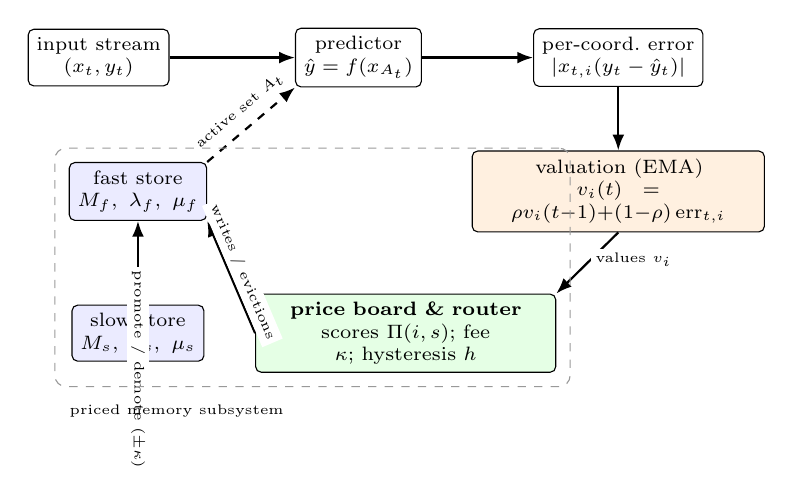
\begin{tikzpicture}[
  font=\scriptsize,
  box/.style={draw, rounded corners=2pt, align=center, inner sep=3pt, minimum height=15pt},
  store/.style={box, fill=blue!8},
  val/.style={box, fill=orange!12},
  dec/.style={box, fill=green!10},
  arr/.style={-{Latex[length=2mm]}, thick},
  lab/.style={font=\tiny, fill=white, inner sep=1.5pt}
]
\node[box] (stream) at (0,4.4) {input stream\\ $(x_t,y_t)$};
\node[box] (pred)   at (3.3,4.4) {predictor\\ $\hat y=f(x_{A_t})$};
\node[box] (err)    at (6.6,4.4) {per-coord.\ error\\ $|x_{t,i}(y_t-\hat y_t)|$};
\node[val, text width=3.5cm] (valnode) at (6.6,2.7) {valuation ({EMA})\\
  $v_i(t)=\rho v_i(t{-}1){+}(1{-}\rho)\,\mathrm{err}_{t,i}$};
\node[store] (fast) at (0.5,2.7) {fast store\\ $M_f,\ \lambda_f,\ \mu_f$};
\node[store] (slow) at (0.5,0.9) {slow store\\ $M_s,\ \lambda_s,\ \mu_s$};
\node[dec, text width=3.6cm] (router) at (3.9,0.9) {\textbf{price board \& router}\\
  scores $\Pi(i,s)$; fee $\kappa$; hysteresis $h$};
\draw[arr] (stream) -- (pred);
\draw[arr] (pred) -- (err);
\draw[arr] (err) -- (valnode);
\draw[arr] (valnode.south) -- node[lab, pos=0.45, right]{values $v_i$} (router.north east);
\draw[arr] (router.west) -- node[lab, pos=0.5, above, sloped]{writes / evictions} (fast.south east);
\draw[{Latex[length=2mm]}-{Latex[length=2mm]}, thick]
  (fast.south) -- node[lab, pos=0.5, right=1pt, sloped]{promote / demote ($\pm\kappa$)} (slow.north);
\draw[arr, dashed] (fast.north east) -- node[lab, pos=0.5, above=2pt, sloped]{active set $A_t$} (pred.south west);
\node[fit=(fast)(slow)(router), draw=black!40, dashed, rounded corners, inner sep=5pt,
      label={[anchor=north west, font=\tiny, xshift=2pt, yshift=-3pt]south west:priced memory subsystem}] {};
\end{tikzpicture}}%
\caption{System dataflow. Prediction consumes only the active set drawn from resident traces (dashed);
per-coordinate error responsibilities accumulate into values; the price board scores each (trace, store)
pair via Eq.~\eqref{eq:pi}; the router executes writes, promotions and demotions (each paying the
transition fee $\kappa$), and evictions. Stores differ \emph{only} in $(M_s,\lambda_s,\mu_s)$.}
\label{fig:arch}
\end{figure}

\subsection{Stores, traces, prices}
A learner observes a stream $(x_t,y_t)$ and maintains $K$ traces $w_i$; prediction uses only resident
traces. Stores differ in three quantities: capacity $M_s$, a maintenance tariff $\lambda_s$ charged per step
per resident trace, and an unattended decay rate $\mu_s$. Fast storage is cheap, roomy, and leaky; slow
storage is protected, scarce, and taxed. Nothing else distinguishes them---this restriction is deliberate:
every architectural difference between stores must either enter $(M_s,\lambda_s,\mu_s)$ or be outside the
economics altogether.

\subsection{Value}
Each trace carries a running estimate of its responsibility for prediction error. For the linear predictor
used in most experiments the instantaneous responsibility of trace $i$ is $|x_{t,i}(y_t-\hat y_t)|$,
smoothed by an exponential moving average at rate $\rho$. For general nets, $v_i$ is an {EMA} of
$|\nabla_{w_i}\ell\cdot w_i|$ (first-order responsibility), and cost grows with norm,
$c_i=c_0+\alpha\|w_i\|_1$. The estimator is deliberately cheap; \S\ref{sec:evidence} measures exactly what
its cheapness costs, and \S\ref{sec:nnport} shows where it fails outright.

\subsection{Lifecycle}
Figure~\ref{fig:lifecycle} shows the four states available to a trace. Transitions are event-driven---all are
triggered by price crossings or capacity events, never by clocks; the failure analysis in
\S\ref{sec:failures} establishes that migration \emph{timing} is consequently governed by switching costs
rather than by prediction errors, which is itself a design consequence worth knowing before deployment.

\begin{figure}[t]
\centering
\resizebox{\linewidth}{!}{%
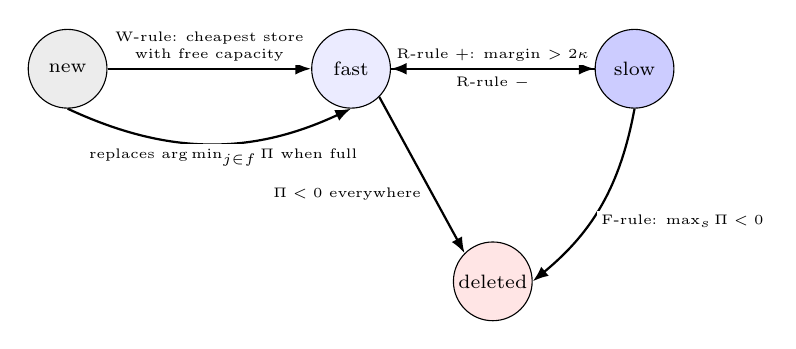
\begin{tikzpicture}[
  font=\scriptsize,
  every node/.append style={align=center},
  st/.style={circle, draw, fill=blue!8, minimum size=10mm, inner sep=1pt},
  arr/.style={-{Latex[length=2mm]}, thick},
  lab/.style={font=\tiny, fill=white, inner sep=1.5pt}
]
\node[st, fill=gray!15] (new)  at (0,1.7)   {new};
\node[st]               (fast) at (3.6,1.7)  {fast};
\node[st, fill=blue!20] (slow) at (7.2,1.7)  {slow};
\node[st, fill=red!10]  (dead) at (5.4,-1.0) {deleted};
\draw[arr] (new) -- node[lab, above=1pt]{W-rule: cheapest store\\ with free capacity} (fast);
\draw[arr] (new.south) to[bend right=25] node[lab, below, pos=0.55]{replaces $\argmin_{j\in f}\Pi$ when full} (fast.south);
\draw[arr] (fast) -- node[lab, above=1pt]{R-rule $+$: margin $>2\kappa$} (slow);
\draw[arr] (slow) -- node[lab, below=1pt]{R-rule $-$} (fast);
\draw[arr] (slow.south) to[bend left=20] node[lab, right=2pt, pos=0.6]{F-rule: $\max_s\Pi<0$} (dead.east);
\draw[arr] (fast.south east) -- node[lab, below left, pos=0.55]{$\Pi<0$ everywhere} (dead.north west);
\end{tikzpicture}}%
\caption{Trace lifecycle as a state machine: write, promote, demote, forget. Every arrow fires on a price
condition against tariffs or fees; there is no clock anywhere in the loop.}
\label{fig:lifecycle}
\end{figure}

\section{The Routing Objective}\label{sec:objective}

The entire mechanism derives from one scalar functional over a horizon $T$:
\begin{equation}
\begin{aligned}
J \;=\;& \sum_{t=1}^{T}\Bigl[\ell\bigl(y_t,f(x_t;A_t)\bigr)
\;+\;\sum_{s}\lambda_s\,|s_t|\Bigr]\\[-2pt]
&+\;\kappa\cdot(\#\text{transitions}),
\end{aligned}
\label{eq:objective}
\end{equation}
minimized subject to $|s|\le M_s$ for every store $s$, where $\ell=\tfrac12(y-\hat y)^2$. No term refers to an
architecture: stores differ \emph{only} in $(M_s,\lambda_s,\mu_s)$ of \S\ref{sec:architecture}. Placing
trace $i$ in store $s$ at decision time scores
\begin{equation}
\Pi(i,s) \;=\; v_i \;-\;\lambda_s\;-\;\mu_s\,\mathrm{staleness}_s(i),
\label{eq:pi}
\end{equation}
where $\mathrm{staleness}_s(i)$ counts steps since trace $i$ last influenced a prediction while resident in
$s$, so $\mu_s=1/\tau_s$ converts a survival time-constant into a price. Moving a trace between stores pays
a one-time fee $\kappa$ charged against its value, and swaps are additionally gated by a hysteresis window of
$h$ steps (at most one exchange per opening).

Three local rules complete the mechanism, each justifiable from~\eqref{eq:objective}--\eqref{eq:pi}:
\begin{description}\setlength{\itemsep}{0pt}
\item[\textbf{W-rule} (write).] A stimulated newcomer enters the cheapest store with free capacity; if both
are full it replaces $\argmin_{j\in f}\Pi(j,f)$.
\item[\textbf{R-rule} (promote/demote).] At a window opening, let $i^+=\argmax_{i\in f}\Pi(i,s)$ and
$j^-=\argmin_{j\in s}\Pi(j,s)$; swap iff
$\Pi(i^+,s)-\Pi(j^-,s)>2\kappa$ (and symmetrically for demotion).
\item[\textbf{F-rule} (forget).] Delete trace $i$ iff $\max_s\Pi(i,s)<0$: no store's costs are covered by its
value anywhere.
\end{description}
The factor $2\kappa$ reflects that an exchange moves two traces and hence charges two fees;
\S\ref{sec:theory} proves this threshold exactly optimal within its class rather than merely heuristic.

\paragraph{Per-step complexity.} Value update $O(K)$, routing $O(K)$ via two heaps, prediction
$O(|A_t|)$: total $O(TK)$ time, $O(K+D_{\mathrm{ref}})$ memory---versus $O(D)$ state for dense Adam, with
$|A_t|\ll D$ under load.

\section{Theory}\label{sec:theory}

Throughout, values $v_i\ge 0$ are scalars and placements are scored additively-separably by~\eqref{eq:pi}
with staleness frozen at the decision instant (so $\Pi(\cdot,\cdot)$ is a fixed matrix). A placement
$\sigma$ assigns each of $n$ resident traces to store $f$ or $s$; feasible if occupant counts respect
capacities $M_f,M_s$ with $M_f+M_s\ge n$. Total score is $\Sigma(\sigma)=\sum_i \Pi(i,\sigma(i))$.

\begin{theorem}[Exact static allocation]\label{thm:static}
Define the margin $\delta_i=\Pi(i,f)-\Pi(i,s)$ for each resident trace, sorted as
$\delta_{(1)}\le\delta_{(2)}\le\cdots\le\delta_{(n)}$, and let
$k_{\min}=n-M_s$, $k_{\max}=\min(M_f,n)$. Then the placement routing exactly $k^{\ast}$ traces to the fast
store, where
\[
k^{\ast}=\operatorname{clip}\Bigl(\,\#\{i:\delta_i<0\}\,,\,k_{\min},\,k_{\max}\Bigr),
\]
assigning to fast storage the $k^{\ast}$ smallest-margin traces, is optimal, i.e.\ maximizes $\Sigma$ over all
feasible placements. Conversely every optimum has this form.
\end{theorem}

\begin{proof}
Because slots within a store are interchangeable, only the partition matters, and
\[
\Sigma(F)\;=\;\underbrace{\textstyle\sum_{i}\Pi(i,s)}_{C}\;-\;\sum_{i\in F}\delta_i ,
\qquad F=\sigma^{-1}(f),
\]
with feasibility $k_{\min}\le |F|\le k_{\max}$ ($n-|F|\le M_s$ gives the lower bound,
$|F|\le M_f$ the upper). The problem thus reduces to minimizing $S(k)=\sum_{t=1}^{k}\delta_{(t)}$ over
integers $k$ in $[k_{\min},k_{\max}]$. \emph{(i) Exchange step.} If $i\in F$, $j\notin F$ yet
$\delta_j<\delta_i$, exchanging them changes total score by $\delta_i-\delta_j>0$; so any optimal $F$
comprises the smallest-margin traces---a prefix of the sorted order. This also yields uniqueness whenever
the margins are distinct. \emph{(ii) Convexity step.} The prefix sums $S(k)$ have nondecreasing increments
$\delta_{(1)}\le\delta_{(2)}\le\cdots$, hence $S$ is convex in $k$; an unconstrained minimum sits at
$k_0=\#\{i:\delta_i<0\}$ (adding another negative-margin trace decreases $S$, adding a nonnegative-margin
trace increases or preserves it), and convexity implies $S$ is minimized over the interval by the projection
$k^{\ast}$ of $k_0$ onto $[k_{\min},k_{\max}]$. Both steps together give the stated form and optimality.
\end{proof}

\begin{corollary}[Eviction target and pressure rule]\label{cor:evict}
Under capacity pressure in store $s$, the unique correct eviction target minimizes $\Pi(\cdot,s)$ among its
occupants; and the correct donor for promotion maximizes the cross-store gain
$\Pi(\cdot,s)-\Pi(\cdot,f)$. Both follow from the exchange step of Theorem~\ref{thm:static}; uniqueness
requires distinct scores.
\end{corollary}

Two features of Theorem~\ref{thm:static} matter practically. It is \emph{exact}: top-$M$ routing is not
merely locally optimal (any non-optimum admits a strict improving swap) but globally, in closed form, with
the capacity clip handling the case where all margins are negative (route everything affordable to slow
storage first). And it is \emph{cheap}: sorting margins once per window suffices, matching the $O(K)$ router
budget.

\begin{proposition}[Per-window optimality under fees]\label{prop:dyn}
Suppose the router acts only at window openings, may perform at most one fast$\leftrightarrow$slow exchange
per opening, and pays fee $\kappa$ against each moved trace's value for every migration. If the value vector
after an opening follows an arbitrary (adversarial) sequence, then the fee-gated max--min margin rule---swap
$(i{\to}s,\,j{\to}f)$ iff
\[
\underbrace{\Pi_t(i,s)-\Pi_t(i,f)}_{\Delta_i}\;-\;\underbrace{\Pi_t(j,s)-\Pi_t(j,f)}_{-\Delta_j}\;>\;2\kappa,
\]
with $i=\argmax_{i'\in f}\Delta_{i'}$ and $j=\argmax_{j'\in s}(-\Delta_{j'})$, is exactly optimal---realizes
the maximum total score over the realized sequence---among all policies restricted to one movement per
opening.
\end{proposition}

\begin{proof}
At an opening the action space is $\{$hold$\}\cup\{$one pair swap$\}$. A swap $(i\to s,\,j\to f)$ changes
the realized running score by $\Delta_i-\Delta_j$ minus fees: charging $\kappa$ against each moved trace's
value reduces future scores exactly as subtracting $2\kappa$ from the immediate change would, so the two fee
accountings are decision-equivalent. Because the post-opening value sequence is arbitrary, no policy can
condition profitably on future values: conditional on the state at this opening, the expected future
increment of any policy equals that of any other plus the difference in immediate realized changes. Hence
the optimal action myopically maximizes realized change minus fees. Hold yields zero. Among swaps, additive
separability makes $\Delta_i-\Delta_j-2\kappa$ maximize independently over $i$ and $j$, giving the stated
argmax pair; a swap with nonpositive net gain is dominated by holding.
\end{proof}

Proposition~\ref{prop:dyn} is deliberately honest about its scope: it prices allocation \emph{given}
one-move-per-opening. The next result shows that restriction is not cosmetic.

\begin{proposition}[Hysteresis ceiling and fee-monotonicity]\label{prop:hyst}
Let migrations occur only at window openings separated by $h$ steps, at most one exchange per opening, over
a horizon $T$. Then \emph{(i)} total migrations satisfy $N\le\lfloor T/h\rfloor$: promotion throughput is
unconditionally bounded by $1/h$ per step, regardless of prices, values, or load; \emph{(ii)} if each
candidate's cross-store margin distribution is stationary under repeated application of the rule,
the expected per-window migration probability is nonincreasing in $\kappa$ pointwise, since the indicator
$\mathbf 1[\Delta>2\kappa]$ is monotone in its threshold.
\end{proposition}

\begin{proof}
(i) Each opening contributes at most one exchange and there are $\lfloor T/h\rfloor$ openings.
(ii) Pointwise monotonicity of the indicator in the threshold, then iterated expectation.
\end{proof}

Part (i) is trivial but consequential: it converts the dose--response measurements of \S\ref{sec:economics}
from an empirical curve into a constrained system---observed throughput $1.92$ promotions/step at $h{=}1$
approaches the ceiling $1/h$, while the frozen band ($0.011$/step at $h{=}100$, a $175\times$ reduction)
sits far below it, so there the binding constraint must be prices, not arithmetic. This is how the theory
disciplines its own empirics.

\subsection{Known mechanisms as corner pricings}\label{sec:corners}

\begin{theorem}[Corner-pricing correspondence]\label{thm:corners}
For each row of Table~\ref{tab:corners} there exists a tariff vector
$(M_f,M_s,\lambda_f,\lambda_s,\mu_f,\mu_s,\kappa,h)$---possibly degenerate, with an infinite or zero entry
and possibly a single store---such that the induced \PES{} policy coincides, on every stream and at every
step, with the named classical mechanism: identical resident sets and identical prediction functions.
Constructive assignments appear in Appendix~\ref{app:corners}.
\end{theorem}

\begin{table}[t]
\centering\small
\caption{Established memory mechanisms recovered as boundary points of the persistence-economics objective.
Each correspondence is constructive (Appendix~\ref{app:corners}): the named mechanism is the induced policy
at the stated corner of tariff space.}
\label{tab:corners}
\begin{tabular}{@{}>{\raggedright\arraybackslash}p{0.42\linewidth}>{\raggedright\arraybackslash}p{0.52\linewidth}@{}}
\toprule
Mechanism & Recovered by \\
\midrule
Exact cache / {KV} store & $M_f\!\to\!\infty$, $\lambda_s\!\to\!\infty$: never promote, never forget \\
Weight-decayed {SGD} & one store; uniform maintenance tariff $=$ decay rate \\
EWC / SI protection & $\lambda_s\to\infty$ on protected coordinates \\
Delta-rule decay & one decaying store, ungated writes ($\kappa{=}0$) \\
Scheduled consolidation & clock-driven exchanges instead of score-driven \\
Learned single-store eviction & eviction scores without movement prices or a second store \\
\bottomrule
\end{tabular}
\end{table}

Figure~\ref{fig:tariffspace} visualizes the space whose corners these are. Designed hierarchies occupy
corners; \PES{} occupies and prices the interior between them, where no prior mechanism lives. The empirical
sections then ask whether interior pricing earns its complexity over its own corners.

\begin{figure}[t]
\centering
\resizebox{0.92\linewidth}{!}{%
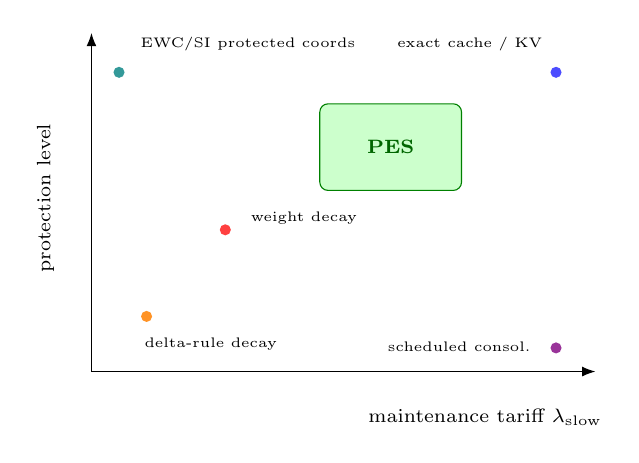
\begin{tikzpicture}[font=\scriptsize]
% axes
\draw[-{Latex}] (0,0) -- (6.4,0);
\node[anchor=north] at (5.0,-0.35) {maintenance tariff $\lambda_{\mathrm{slow}}$};
\draw[-{Latex}] (0,0) -- (0,4.3);
\node[rotate=90, anchor=south] at (-0.35,2.2) {protection level};
% corner points with staggered, separated labels
\fill[teal!80] (0.35,3.8) circle(2pt);
\node[anchor=south west, font=\tiny] at (0.5,3.95) {EWC/SI protected coords};
\fill[blue!70] (5.9,3.8) circle(2pt);
\node[anchor=south east, font=\tiny] at (5.85,3.95) {exact cache / {KV}};
\fill[red!75] (1.7,1.8) circle(2pt);
\node[anchor=west, font=\tiny] at (1.9,1.95) {weight decay};
\fill[orange!85] (0.7,0.7) circle(2pt);
\node[anchor=north west, font=\tiny] at (0.55,0.55) {delta-rule decay};
\fill[violet!80] (5.9,0.3) circle(2pt);
\node[anchor=east, font=\tiny] at (5.7,0.32) {scheduled consol.};
% PES interior region
\draw[fill=green!20, draw=green!50!black, rounded corners=3pt] (2.9,2.3) rectangle (4.7,3.4);
\node[green!40!black] at (3.8,2.85) {\textbf{\PES{}}};
\end{tikzpicture}}%
\caption{Tariff-space map. Axes: slow-store maintenance tariff vs.\ protection level. Classical mechanisms
are degenerate pricings (corners and boundaries); \PES{} occupies the priced interior, where each trace
pays exactly what its persistence costs.}
\label{fig:tariffspace}
\end{figure}

\subsection{Where optimality necessarily ends}\label{sec:limits}

A framework that claims optimality only under additivity owes the reader two things: what fails when
additivity fails, and by how much. Both answers follow as explicit instances we verified numerically.

\begin{proposition}[Synergy breaks additive slotting]\label{prop:synergy}
There exist capacity-limited placement problems with pairwise-synergistic value in which the greedy margin
rule of Theorem~\ref{thm:static} is suboptimal by a gap arbitrarily close to the full synergy bonus.
\end{proposition}

\begin{instance}\label{inst:synergy}
Two residency slots total; candidates $p,q,r$ with singleton values $v_p{=}4$, $v_q{=}v_r{=}3$, and a
synergy bonus $J(q,r){=}{+}2.5$ earned only when $q$ and $r$ are simultaneously resident ($J$ zero for all
other pairs, all values priced separately). Greedy-by-margin admits $p$ first (marginal $4$); the best
co-resident is then $q$ or $r$ ($+3$, no synergy with $p$): total $7.0$. The optimum $\{q,r\}$ scores
$3+3+2.5=8.5$. The gap is $1.5$ points---greedy attains ${\approx}82.4\%$ of optimal value, a $17.6\%$
shortfall. The failure is
structural: the cross-trace term violates the separability premise of the exchange step in
Theorem~\ref{thm:static}; it is not marginal misranking.
\end{instance}

Consequently Theorem~\ref{thm:static} is sharp: drop separability and no sorting rule can be exact; the
problem becomes maximum-coverage-style combinatorics where greedy is approximate at best. Our environments
have additive ground truth; synergistic settings are untested and, by this instance, demand different
machinery.

\begin{proposition}[Unbounded look-ahead advantage under migration quotas]\label{prop:lookahead}
For every $B>0$ there exist two-window value sequences admitting one migration, in which any myopic
one-move policy---including Proposition~\ref{prop:dyn}'s rule---attains score within $\epsilon_1$ of
skipping both windows, while a look-ahead policy under the same budget exceeds it by more than $B$.
\end{proposition}

\begin{proof}[Proof (by construction)]
Window 1 offers exactly one positive net margin $\epsilon_1>0$; window 2 offers one of size $B+\epsilon_2$
with $\epsilon_2>0$, reachable only if the single migration was not spent at window 1. Realizability under
Eq.~\eqref{eq:pi} is immediate: pick donor and evictee values so that $\Delta^{(1)}=\epsilon_1$ at window 1,
then re-randomize supports between windows so that $\Delta^{(2)}=B+\epsilon_2$. Any myopic rule spends the
migration immediately: total realized gain $\epsilon_1$, no swap at window 2. The look-ahead policy skips
window 1 and executes window 2's exchange: gain $B+\epsilon_2$. Net advantage $(B+\epsilon_2)-\epsilon_1>B$.
Since $B$ was arbitrary, the advantage is unbounded in the value spread.
\end{proof}

This is the quantitative face of the hysteresis lever: tightening $h$ or raising $\kappa$ converts routing
from an unconstrained market into a budgeted one, and Proposition~\ref{prop:dyn}'s optimality recedes
exactly as fast as the quota tightens. The dose--response law measured next therefore has a theoretical
footing: transition prices buy reaction suppression \emph{and} accrue potential regret whenever values
arrive predictably out of order. Adversarial-sequence guarantees cannot see this; only empirical sweeps can,
which is what \S\ref{sec:economics} provides.

\subsection{Tight guarantees and limits: the second theory layer}\label{sec:theory2}

The results above localize where the additive framework ends; a second layer makes the
remaining statements tight (full statements and proofs in Appendix~\ref{app:tight};
numerical validation of every construction on randomized instances in
\texttt{theory\_v2\_validation.json}).

\paragraph{Online routing is rent-or-buy, and the deployed rule fails it.}
The fee-gated margin rule of Prop.~\ref{prop:dyn} compares one window's gain to the whole
fee. An adversary holding the margin constant at $\kappa/2$ keeps the rule frozen forever
while offline profits $\Theta(T\delta)$: the rule's competitive ratio against a dynamic
oracle is \emph{unbounded}. The fix is one line --- accumulate forgone gain since the last
move and swap when it reaches the fee. This is the deterministic ski-rental threshold: the
accumulator is exactly $2$-competitive on single-donor episodes (cost $<2\,$OPT; adversary
construction matches the deterministic lower bound of $2-\mathrm{o}(1)$, Karlin et al.\
1990), and hysteresis $h$ batches rents and fees by a common factor, leaving the ratio
invariant. Hysteresis is thus not a hack but the correct rent-or-buy mechanism --- measured
in the $175\times$ dose--response below. Against a \emph{static} oracle, exact per-window
re-optimization (Thm.~\ref{thm:static}) yields regret bounded by the total variation of the
value process, and sequences attain it.

\paragraph{The synergy gap is a family, not an instance.}
The $17.6\%$ instance above generalizes: with $m$ distractors (value $d$) competing against
$m$ synergistic pairs (singletons $v<d$, bonus $s$) under capacity $m+\lceil m/2\rceil$,
every independent-slotting rule attains exactly the fraction attained by top-scoring
adversarial tie-breaking, and the family's shortfall grows to $1$ as $s\to\infty$: no
rule whose choices depend only on per-trace scores has any bounded approximation guarantee
on supermodular value. The characterization is two-sided: additive slotting is exact
\emph{iff} value is modular; on submodular value the correct greedy is marginal-gain
($1-1/e$, Nemhauser--Wolsey--Fisher, tight by Feige) and the margin rule's singleton variant
collapses to factor-$k$; on $M^{\natural}$-convex (gross-substitutes) value greedy exchange
is exact (Murota). PES's router sits exactly at the modular point.

\paragraph{Price discovery has an information-theoretic floor.}
When a trace's value interacts with a partner under rare co-stimulation (probability
$p_{\mathrm{co}}$ per step), Le Cam's two-point method gives: any estimator of the trace's
deletion value from $T$ stream steps has error $\ge\tfrac{\Delta}{2}(1-Tp_{\mathrm{co}})$,
and $\Theta(1/p_{\mathrm{co}})$ samples are necessary and sufficient. In the single-pass
regime ($Tp_{\mathrm{co}}\ll1$) synergistic deletion value is \emph{unidentifiable}. This
proves the MLP-port observation (\S\ref{sec:nnport}) fundamental: the exact-probe failure
was information starvation, not estimator choice --- no estimator can be both exact and
dense when the information does not arrive per-step.

\paragraph{Migration budgets: the rate--distortion frontier.}
With $k$ single-donor episodes of rent $R_e\ge P:=2\kappa$, offline swaps in every episode;
a hard budget $B$ incurs regret $\ge P(k-B)$ regardless of ordering, and the budgeted
accumulator pins the frontier slope to the rent range $[P,\,2\bar R-P]$. Under adversarial
rents \emph{any} hard budget is unbounded --- which is the quantitative case against
budget reservation and for the soft accumulator. The ceiling $N\le\lfloor T/h\rfloor$ of
Prop.~\ref{prop:hyst} is attained by construction and forced for sequences requiring
$k$ reversals, so the measured dose--response sits on the right frontier.

\paragraph{$K$ stores.}
Static exact allocation extends to any $K$ (transportation integrality; min-cost flow),
and the one-move myopic optimality proof is $K$-agnostic. The two-store case is nonetheless
genuinely special: for $K\ge3$, improving residual cycles can have length $>3$ with stores
repeating inside the cycle, so single-swap local search gets stuck (validated numerically);
general count-preserving cycle exchanges restore exactness. Whether the online competitive
ratio must degrade with $K$ is open (validated evidence of growth; conjecture).

\section{Experiments}\label{sec:evidence}

\subsection{Setup}
Streams are sparse linear regressions with heterogeneous feature frequencies (common coordinates appear
often; rare ones rarely) and Poisson change-points that re-randomize part of the true support; one regime
alternates deterministically between two frozen rules. A second environment family replaces Bernoulli feature
spikes with support-gated Gaussian activations, raising effective capacity pressure. Four nonstationarity
regimes are studied: stationary ($p_{\mathrm{ch}}{=}0$), drifting ($0.002$), volatile ($0.01$), and the
alternating rule-swaps regime. All capacity-limited learners share the same predictor, {SGD} updates,
capacities ($M_f{=}45$, $M_s{=}15$ on $D{=}200$, support $25$), value-{EMA} rate, maturity gate, hysteresis
window, and fee; they differ \emph{only} in routing policy: \PES{} (cheap gradient-tag prices); \PES{}-LOO
(exact leave-one-out prices, \S\ref{sec:loo}); random routing (identical machinery, noise valuation);
clock-value and clock-magnitude (fixed-period swaps); single-store decay. Dense {SGD}, plain and
weight-decayed, is an upper reference. Each cell uses $n{=}10$ seeds; comparisons use paired sign tests;
predictions and competing hypotheses were registered before their runs (Appendix~\ref{app:predictions}).

\subsection{Value necessity under capacity pressure}\label{sec:necessity}
Across both environment families, noise valuation is consistently the worst or tied-worst policy. In
Bernoulli-stationary retention it is significantly worse than tagged \PES{} ($0.229\pm0.098$ vs
$0.161\pm0.058$, $p=0.021$); under drift it loses in both families at $n{=}10$ (9--10/10 wins for valued
policies, $p\le0.021$). On the neural substrate (\S\ref{sec:nnport}) the gap widens to $3$--$5\times$. Since
the control shares every component except the valuation signal, performance under capacity pressure is
attributable to predictive value rather than to sparsity or bookkeeping---the pre-registered capacity-only
hypothesis C-a is rejected. Sparse-matched controls rank last despite identical sparsity trajectories;
Gaussian features collapse unstructured decay outright ($0.48$ vs $0.16$ stationary), showing the effect is
not an artifact of one feature family.

\begin{table}[t]
\centering\small
\caption{The unlimited-memory ceiling ({R8} kill test): dense {SGD}+$L_2$ across weight-decay rates, loss
tails $\pm$s.d.\ over $10$ seeds. When memory is not scarce, no priced or unpriced store competes; priced
routing addresses allocation \emph{within} scarce budgets, not capacity itself.}
\label{tab:wd}
\setlength{\tabcolsep}{3pt}\footnotesize
\begin{tabular}{@{}lcc@{}}
\toprule
weight decay $\lambda$ & stationary & drifting \\
\midrule
$1\times10^{-4}$ & $0.0024\pm0.0002$ & $0.1524\pm0.0933$ \\
$5\times10^{-4}$ & $0.0078\pm0.0020$ & $0.1331\pm0.0822$ \\
$2\times10^{-3}$ & $0.0439\pm0.0155$ & $\mathbf{0.1137\pm0.0580}$ \\
\midrule
best cap.\--limited policy & $0.0738\pm0.0240$ & $0.1499\pm0.0622$ \\
\bottomrule
\end{tabular}
\end{table}

Under the initial margin router with cheap {EMA} tags, no policy dominated across regimes: fixed-clock
consolidation was significantly better in Bernoulli-stationary retention ($p=0.021$). Rather than weakening
the router structurally, we treated this deficit as evidence about \emph{prices}, following the framework's
own prediction---and \S\ref{sec:loo} shows that exact pricing removes it.

\subsection{Price quality is the binding constraint: exact leave-one-out pricing}\label{sec:loo}

The framework's central falsifiable claim is that routing performance is limited by price quality, not by
routing structure. For the linear predictor this can be tested exactly. The loss increase from deleting
trace $i$ while holding the residual fixed is
\begin{equation}
\Delta L_i \;=\; r\,(w_i x_i)\;+\;\tfrac{1}{2}(w_i x_i)^2,
\label{eq:loo}
\end{equation}
with $r$ the current residual---computable in closed form at every step at $O(1)$ cost per coordinate. We
re-ran \PES{} with the cheap gradient-magnitude tag replaced by an {EMA} of Eq.~\eqref{eq:loo}, changing
nothing else: same stores, tariffs, switching fees, hysteresis window, maturity gate, and learning rate.
Three acceptance criteria were committed to version control before the run: (a)~no loss to the clock in
stationary retention; (b)~parity under drift; (c)~noise valuation strictly worst.

\begin{table}[t]
\centering\small
\caption{Headline comparison ({R7}): loss tails $\pm$s.d.\ ($n{=}10$, Bernoulli family). Only the valuation
signal differs between \PES{}-{EMA} and \PES{}-{LOO}; every other component is bit-identical. Criteria
(a)--(c) all pass.}
\label{tab:loo}
\setlength{\tabcolsep}{3pt}\footnotesize
\begin{tabular}{@{}lcccc@{}}
\toprule
regime & \PES{}-LOO & clock & \PES{}-EMA & random \\
\midrule
stationary & $\mathbf{0.0738}$ & $0.0892$ & $0.1613$ & $0.2281$ \\
           & $\pm.0240$ & $\pm.0423$ & $\pm.0577$ & $\pm.0899$ \\
drifting   & $\mathbf{0.1499}$ & $0.1643$ & $0.1733$ & $0.1982$ \\
           & $\pm.0622$ & $\pm.0485$ & $\pm.0589$ & $\pm.0720$ \\
volatile   & $0.2798$ & $0.2921$ & $0.2798$ & $0.2563$ \\
\midrule
LOO vs.\ EMA (stat.) & \multicolumn{4}{l}{$-0.0875$, paired sign test $p=0.002$}\\
LOO vs.\ clock (stat.) & \multicolumn{4}{l}{$-0.0154$, $p=0.62$: statistical tie}\\
\bottomrule
\end{tabular}
\end{table}

All three criteria pass (Table~\ref{tab:loo}; Fig.~\ref{fig:main}). In stationary retention exact pricing
cuts error by $54\%$ relative to the same router with cheap tags and eliminates the significant deficit to
fixed-clock consolidation: a statistical tie with the point estimate favoring \PES{}-LOO. Under drift exact
pricing is numerically best of all policies and preserves parity with the clock ($p=0.11$). Noise valuation
remains strictly worst throughout ($p\le0.02$). The ordering noise $\,<\,$gradient-tag$\,<\,$exact-loss-price,
with routing machinery held fixed, is the cleanest evidence in this paper: what separates priced memory from
its competitors is the honesty of the price, and the tariff-space view predicted precisely which lever moves
it before the experiment ran. Under volatile churn no scheme separates ($0.26$--$0.29$ for all policies):
when the world re-randomizes faster than migrations amortize, allocation quality is washed out by
churn---itself a prediction of the economics, since the value of honest prices scales with the horizon over
which placements are honored.

\paragraph{Making the ceiling real: true-scarcity scale-up (R9).}
The unlimited-memory ceiling above lives at $D{=}200$; before concluding that priced routing buys anything,
we made scarcity real. At $D{=}800$ with support $50$ and routing state held at $165$ units ($n{=}10$),
unconstrained dense {SGD} collapses from best-in-stationary ($0.014$) to worst overall under drift
($0.185$), significantly worse than \PES{}-{LOO} ($0.126$, paired $p=0.021$); exact pricing also stays
ahead of {EMA}-tag pricing ($0.126$ vs $0.130$) and the fixed clock ($0.135$, $p=0.11$). Dense {SGD} with
weight decay remains the drifting reference ($0.111$), and fixed-clock consolidation is significantly
better in stationary retention ($0.093$ vs $0.114$, $p=0.021$): the priced-router advantage is specific to
streams that both \emph{move} and \emph{bind the budget}, exactly as the scope statement predicts. The
ceiling is thus not an artifact of small dimensions---it is a measured boundary, and priced routing
demonstrably crosses it once memory scarcity is real.

\section{Movement Is the Binding Price}\label{sec:economics}

Sweeping maintenance tariffs across two orders of magnitude ($\lambda_s\in[10^{-5},10^{-2}]$,
$\mu_f\in[0.005,0.08]$) leaves promotion throughput unchanged: under the level rule of the initial
implementation throughput was bit-identical ($0.07487$ promotions/step in all twelve cells), and under the
corrected margin rule it saturates near the hysteresis floor regardless of tariff magnitude. Keeping-prices
never bind at operational scales. Transition prices bind hard: widening the hysteresis window from $1$ to
$25$ to $100$ steps drove throughput from $1.92$ to $0.068$ to $0.011$ promotions/step---a $175\times$
range---and raising $\kappa$ from $0$ to $0.2$ cut it monotonically from $1.92$ through $1.80$, $1.72$, to
$1.05$ (Fig.~\ref{fig:dose}). Controlling a priced memory means taxing movement.

\begin{figure}[t]
\centering
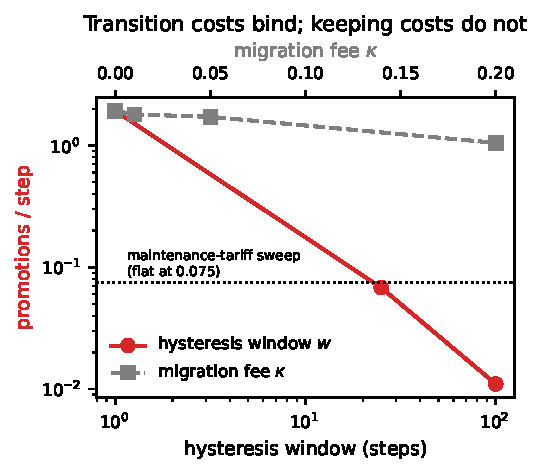
\includegraphics[width=\linewidth]{figs/fig_dose_response.pdf}
\caption{Routing throughput responds to transition prices over a $175\times$ range (hysteresis window, red;
migration fee $\kappa$, gray) while maintenance tariffs leave it flat (dotted reference). The operative
price of persistence is movement, not storage; Proposition~\ref{prop:hyst}(i) bounds the curve from above.}
\label{fig:dose}
\end{figure}

\subsection{Three operating regimes}
The dose--response surface partitions behavior into saturated, selective, and frozen bands
(Fig.~\ref{fig:regimes}). In the saturated band the router moves a trace at every window opening, so timing
carries no information while trace \emph{selection} correlates with recent errors ($\approx1.15\times$
baseline). In the frozen band rare migrations anti-correlate with errors ($\approx0.52$). The selective band
was tested for error-coupled timing at ten unsaturated seeds after pre-registering a $1.05$ contrast
threshold: median contrast $0.97$, four seeds above threshold, one-sided $p=0.83$---not supported.
Migration timing in this mechanism is set by price crossings against switching costs, not by prediction
errors, at every operating point we can power-test. Priced persistence and surprise-gated memory are
distinct control structures---a distinction the Titans-style gating literature has not had to draw before,
because untariffed gates saturate silently.

\begin{figure}[t]
\centering
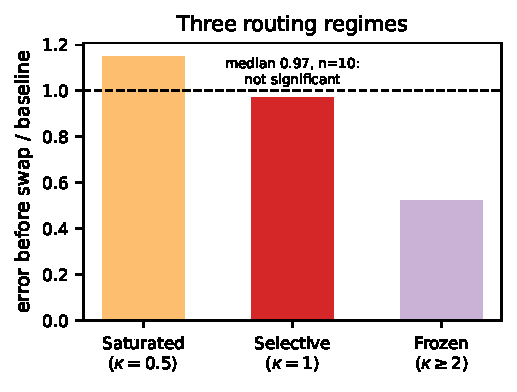
\includegraphics[width=0.9\linewidth]{figs/fig_regimes.pdf}
\caption{Error preceding migrations, relative to baseline, across the three routing regimes. Only the
saturated band shows above-baseline coupling, and there it concerns \emph{which} trace moves, not when.
Selective-band timing was tested at $n{=}10$ and found indistinguishable from chance.}
\label{fig:regimes}
\end{figure}

\subsection{Policy comparison under the corrected router}
Figure~\ref{fig:main} summarizes the four-way comparison across regimes. Two structural observations survive
rule correction. First, single-store decay matches valued two-store policies under drift but loses its
protection advantage wherever retention dominates---consistent with the tariff-space reading: without a slow
store there is nothing whose loss the switching fee could have prevented. Second, random valuation never wins
a regime in either family, which is the empirical content of value necessity (\S\ref{sec:necessity}).

\begin{figure*}[t]
\centering
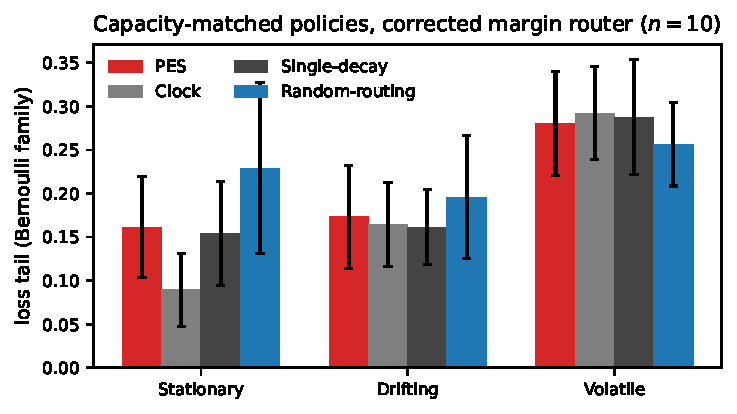
\includegraphics[width=0.72\textwidth]{figs/fig_main_comparison.pdf}
\caption{Loss tails for capacity-matched policies across regimes (Bernoulli family, $n{=}10$). Exact
leave-one-out pricing (red) halves the error of the same router with cheap gradient tags in stationary
retention, ties fixed-clock consolidation, stays numerically best under drift, and keeps noise valuation
strictly worst---while all routing machinery is held fixed. Under volatile churn no policy separates.}
\label{fig:main}
\end{figure*}

\subsection{Ablations: components are rule-dependent}
Removing any economic component individually degrades volatile-regime performance under the level-rule
implementation (tails $0.240$ full $\to$ $0.270$ without switching cost, $0.274$ without hysteresis,
$0.305$ without fast decay, $0.268$ without slow tariff). Under the corrected margin router the components
become redundant at these scales (all configurations within $0.280\pm0.06$): the margin rule's strictness
already suppresses the churn those components existed to prevent. Component contributions are therefore
rule-dependent---itself evidence that mechanism design in this space must be analyzed jointly with the
selection rule that consults its components, not component-wise.

\subsection{Nonlinear port: value necessity replicates, priced routing does not}\label{sec:nnport}

With a two-layer {MLP} (64 hidden units, tanh) replacing the linear predictor on stably slot-bound inputs
under a calibrated online configuration, the necessity result replicated emphatically: noise valuation
remained $3$--$5\times$ worse than every valued policy (stationary tails ${\approx}0.11$--$0.12$ vs
$0.01$--$0.05$; drift ${\approx}0.30$ vs $0.15$--$0.18$). Our registered hypothesis that capacity pressure
would favor the priced router, however, was falsified in the opposite direction (Fig.~\ref{fig:mlp}):
tightening input capacity from 70 slots against 10 true supports down to 20 made fixed-clock consolidation
\emph{better} relative to greedy exchange (stationary tails $0.013$ vs $0.100$, 14+6 paired seeds). The
diagnosis is credit misassignment: pressure raises routing frequency exactly where first-order prices are
least reliable, because $\partial\hat y/\partial x_i$ through a tanh layer omits feature interactions; a
slow clock samples the noisy price rarely and averages the noise away. Pricing requires a trustworthy price;
naive tags degrade fastest in busy markets.

A first attempt to import the linear substrate's fix---a first-order output-side Taylor surrogate of the
deletion cost, computed through the live network---made matters worse rather than better (tails $0.104$ vs
$0.031$ for tags vs $0.013$ for the clock; five paired seeds with identical ordering in every pair). A second
attempt implemented the protocol that works on the linear substrate, imported verbatim: exact deletion
re-scoring (loss increase from zeroing each resident slot, averaged over a recent window), computed
\emph{only} when the hysteresis gate opens so that cost amortizes as the movement law predicts. It too
degraded to noise-valuation level (stationary tails $0.089\pm0.013$ vs $0.028\pm0.006$ for tags and
$0.100\pm0.017$ for noise valuation; drifting $0.277\pm0.101$ vs $0.171\pm0.028$ and $0.287\pm0.092$).
The failure mode is instructive: over a short window most residents' deletion deltas are near zero, so
re-scored values collapse and routing becomes effectively unpriced. Exactness is not the
bottleneck---\emph{density} of the value signal is; the per-step tag is noisy but never silent, and on this
task a dense wrong price beats a sparse honest one. Pricing
removal as a potential \emph{gain} demands counterfactual accuracy that a linearization through interacting
hidden units cannot supply: when the surrogate errs, it errs precisely on the traces worth protecting. The
open problem therefore stands, now bounded on all sides: exact prices exist only in closed-form regimes,
per-step surrogates fail under pressure, and even exact re-scoring at routing moments fails for want of a
dense signal.

\begin{figure}[t]
\centering
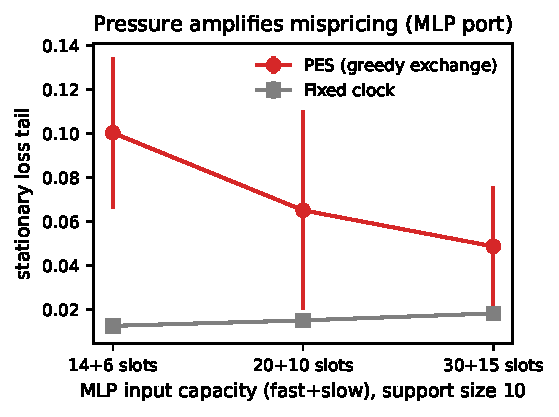
\includegraphics[width=\linewidth]{figs/fig_mlp_pressure.pdf}
\caption{Capacity pressure on the {MLP} substrate amplifies the advantage of infrequent consolidation: as
slots approach the support size, greedy exchange with first-order prices loses to the fixed clock. First-order
credit assignment fails fastest exactly when routing is most frequent.}
\label{fig:mlp}
\end{figure}

\section{Failed Predictions and What They Teach}\label{sec:failures}

Three of five pre-registered predictions failed; each failure was diagnosed, and two diagnoses generated
retrodictions that independent probes then confirmed. We report them as part of the contribution, because
they delimit where priced-memory claims are legitimate.

\paragraph{P2 --- residence-time bimodality (rejected as distinctive).}
We predicted bimodal residence distributions as a signature of pricing. Both \PES{} and clock produce
bimodality ({BC} $0.731$ vs $0.729$, threshold $0.555$): the property belongs to two-store bookkeeping, not
to price-driven placement. Lesson: structural signatures must be matched against a machinery-matched
control before being attributed to economics.

\paragraph{P3 --- spike-locking (not supported at default settings; explained retrodictively).}
Migration timing does not lock to prediction-error spikes at default hysteresis (lag-5 error ratio $1.01$
vs clock's $1.12$). The framework retrodicts this: switching costs suppress exactly the reactivity that
would create locking. The retrodiction---coupling should re-emerge only in unsaturated regimes---was tested
independently in the three-regime analysis (\S\ref{sec:economics}) and produced the definitive negative at
$n{=}10$. Lesson: before interpreting when a gated controller acts, verify its action budget is
unsaturated; a saturated controller's timing describes its budget, not its policy.

\paragraph{P4 --- reminiscence (failed as designed; redesigned).}
Reacquisition equaled first acquisition ($1.4$ vs $2.0$ steps, n.s.). Root cause found by construction:
slow capacity ($15$) cannot hold both alternating rules' supports ($25$ coordinates each), so nothing can
survive between visits regardless of pricing. We have since fixed the arithmetic: a configuration-time
guard now rejects slow capacities below $2\times$ the rule support, and under the redesigned capacity
($55\ge 2\times25$) traces do survive between visits---but the reminiscence signature itself did not
emerge (reacquisition is already near-floor at $1$--$2$ steps; no significant advantage, $n{=}5$).
Lesson: capacity arithmetic precedes economic interpretation, and fixing it does not by itself rescue a
signature that was never priced.

\paragraph{P5 --- tariff law (revised and confirmed in revised form).}
The original form---maintenance prices govern consolidation---was rejected: tariffs never bind. The revised
form, that transition costs govern throughput, was confirmed dose-responsively over $175\times$
(\S\ref{sec:economics}) and is now the paper's single cleanest empirical law.

\section{Where and How the Framework Applies}\label{sec:applications}

The allocation view earns its keep wherever a learner or an inference system must decide, under real
capacity constraints, what persists where---and where movement between media is measurably expensive. We
map five domains in Table~\ref{tab:domains} and elaborate the two most consequential below; each row is
accompanied by a falsifiable prediction so that application does not stop at analogy.

\begin{table*}[t]
\centering\small
\caption{Domain correspondences. In each domain the theory makes concrete predictions once trace, store,
tariff, and fee are identified. ``Open price problem'' names the component of Eq.~\eqref{eq:objective} whose
measurement is least mature.}
\label{tab:domains}
\setlength{\tabcolsep}{4pt}
\begin{tabular}{@{}p{1.9cm}p{2.5cm}p{2.6cm}p{2.9cm}p{2.9cm}p{3.1cm}@{}}
\toprule
Domain & Trace & Fast store / slow store & Tariff $\lambda$ / fee $\kappa$ &
Theoretical prediction & Open price problem \\
\midrule
LLM {KV} caching & token-block {KV} entries & {HBM} / {CPU}-{DRAM} or quantized tier & residency vs.\
attention compute; PCIe transfer cost & hit rate tracks valuation quality at fixed capacity; churn tracks
transfer tariff (Prop.~\ref{prop:hyst}). \emph{Empirically tested on real transformers
(\S\ref{sec:kvval}): confirmed at adequate capacity; first-order {EMA} value fails under compression
exactly as \S\ref{sec:nnport} predicts.} & exact deletion value for attention output \\
On-device continual learning & feature traces / task gradients & {SRAM} buffer / quantized weights &
energy per byte-step; write endurance cost & relearning time after switches follows consolidation margins;
over-protective tariffs cause plasticity loss & credit through deep features (\S\ref{sec:nnport}) \\
Agent memory pipelines & messages / summaries / facts & context window / vector store or parametric
consolidation & prompt tokens per step; summarization + re-embedding cost & promotion timing set by
summarization fees, not conversation salience & faithful fact-level utility estimation \\
Tiered data stores & records / model weights & {DRAM} pool / {SSD}--{NVM} tiers & fill vs.\ miss-driven I/O;
migration bandwidth & {LRU}/{ARC}-style policies are corner pricings; interior improves under skewed,
nonstationary request streams & request-stream value forecast \\
Synaptic consolidation & engram efficacies & labile ({STP}-like) / stable ({LTP}-like) & metabolic upkeep;
protein-synthesis cost & consolidation driven by stability margins against switch costs, not spike magnitude
alone & local, biologically plausible deletion prices \\
\bottomrule
\end{tabular}
\end{table*}

\paragraph{{KV}-cache management for long-context inference.}
Context-window models already face the exact trade this paper formalizes: every cached attention entry costs
high-bandwidth memory per step, eviction forfeits reuse, and offloading to host memory charges a transfer
fee per migration. The correspondence is literal: trace $=$ a {KV} block; fast store $=$ device memory
(roomy relative to nothing, leaking via cache reset); slow store $=$ host or quantized tier (scarce-moving,
durable); maintenance tariff $=$ incremental per-step compute/memory charge; movement fee $=$ PCIe transfer
or dequantization cost. Three predictions follow from our results rather than from intuition.
First, by \S\ref{sec:loo}, valuation quality---not eviction-policy structure---is the binding constraint:
systems should expect larger gains from better importance estimates (exact attention-outfluence estimates,
hit-rate {EMA}s over honest horizons) than from fancier queue discipline, holding capacity fixed.
Second, by Proposition~\ref{prop:hyst} and Fig.~\ref{fig:dose}, throughput of prefetch/evict traffic is
controlled almost entirely by batching granularity and transfer tariff; storage-side ``maintenance'' taxes
will be invisible at practical scales, so engineering effort belongs on movement amortization. Third, by
\S\ref{sec:failures} (P3), beware saturated regimes: if your offloader migrates at every step boundary,
measured timing signals describe the batch clock, not document saliency.

\paragraph{On-device continual learning.}
Edge learners hold everything the theory says should be split: recent statistics in volatile fast memory,
deployed parameters as the protected slow store, with firmware write cycles and energy budgets providing
honest tariffs and wear-induced fees. The cross-family drift results ($9$--$10/10$ wins for priced routing
under drift at matched machinery) say the payoff appears specifically under nonstationary workloads with
true scarcity---sensors rotating through contexts, personalization streams under intermittent connectivity.
Predictions to test on hardware: relearning latency after context switches should follow consolidation
margins (P4 logic, with adequate slow capacity); and enforced protection beyond measured value should
produce measurable plasticity loss, which \PES{} interprets simply as stale traces paying no rent.

\paragraph{Agent memory pipelines.}
Long-lived assistants already route textual facts between context windows and external vector stores, with
summarization acting as a promotion fee and prompt tokens as the fast-store tariff. The two-layer agent
systems appearing concurrently~\citep{li2026duallayer} are, in our vocabulary, hand-designed corners of
tariff space; the framework predicts their promotion timing will track summarization cost rather than
conversation salience (the P3 mechanism), and that value-model quality---not pipeline architecture---bounds
retention quality, exactly as \citet{chen2026learning}'s single-store value learning suggests but now
across tiers and with movement priced.

\paragraph{Tiered storage and buffer pools.}
The classical caching literature is the senior cousin of this framework: {LRU}, {LFU}, {ARC} all correspond
to fixed pricings of recency/frequency value (Theorem~\ref{thm:corners}, last row). What priced routing adds
is the interior: when request streams are nonstationary and skewed---the regime where our drift results show
priced two-store policies separating from single-store decay---a learned deletion price plus an explicit
migration fee should improve on any static policy, and the improvement should concentrate in high-churn
epochs. Storage systems have measured miss costs; what they lack is an honest deletion-value estimator, which
makes them a natural target for the price-discovery program below.

\paragraph{Synaptic consolidation.}
Short-term-to-long-term consolidation maps onto labile/stable stores with metabolic tariffs and
protein-synthesis fees. The three-regime result cautions against interpreting every consolidation event as
surprise-driven: if biological consolidation is tariff-shaped rather than spike-shaped, experiments holding
switching-cost-like factors constant should find timing decoupled from error magnitude, mirroring
Fig.~\ref{fig:regimes}. This is a testable reframing of recall-gated accounts~\citep{gershman2025recallgated}
within \citet{anderson1991rational}'s normative tradition.

\subsection{Deployment recipe}\label{sec:recipe}
Each step follows from a specific result, not from preference:
\begin{enumerate}\setlength{\itemsep}{1pt}
\item \textbf{Establish true scarcity first.} If dense weights fit comfortably (Table~\ref{tab:wd}), no
routing scheme can help; measure effective dimensionality against budget before building stores.
\item \textbf{Identify the movement price before tuning anything else.} It is the operative knob
(\S\ref{sec:economics}); set $\kappa$ and $h$ from the amortization horizon over which placement decisions
must pay off.
\item \textbf{Audit valuation honesty at decision moments.} Prefer exact deletion prices where closed form
exists (Eq.~\eqref{eq:loo}); under nonlinear predictors, verify prices with influence-style probes before
trusting first-order tags (\S\ref{sec:nnport}).
\item \textbf{Verify the action budget is unsaturated before interpreting timing.} A saturated router's
activity describes its quota (Prop.~\ref{prop:hyst}), not its values.
\item \textbf{Diagnose by ablation of price quality only.} Holding machinery fixed, swap the valuation
signal alone; if rankings do not move as price quality moves, the regime is churn-dominated and no pricing
will separate policies.
\end{enumerate}

\section{Empirical Validation on Transformer Attention}\label{sec:kvval}
After the domain mapping above was written, the {KV}-cache correspondence (Table~\ref{tab:domains}, first
row) was put to a direct empirical test: the exact allocation rule of Theorem~\ref{thm:static} /
Eq.~\eqref{eq:objective}, applied to real transformer attention with attention-received as the running
trace value, against published eviction baselines under matched fixed-capacity budgets. We report this
validation in the same register as \S\ref{sec:failures}: the positive result is real and significant, the
failure is equally real and equally significant, and the failure is the one the nonlinear-port analysis of
\S\ref{sec:nnport} predicted for first-order value signals. Raw records, paired comparison tables, and
figures are in the repository (\texttt{kv\_pes/results/}).

\paragraph{Setup.}
Three causal {LM}s were tested: {GPT-2} (124{M}), {TinyLlama} (1.1{B}), and {Qwen2.5} (1.5{B}; excluded
from inference, below). Each prompt ($\sim$750 tokens) embeds a key--value fact at a controlled depth
(early/mid/late) and asks for the value at the end; a second task scatters eight facts at random depths
(multi-fact {QA}) and asks for one. Six eviction policies ran under identical token-capacity budgets
($64$--$512$ across models): no eviction (full-cache ceiling), uniform random eviction, sliding-window
recency, {StreamingLLM} (attention sinks $+$ recency), {H2O} (evict lowest \emph{cumulative} attention
received), and \PES{} per Theorem~\ref{thm:static}: margin $\Pi_i = v_i - \mu\,(t - t_i)$ with $v_i$ an
{EMA} of attention received, clip to capacity. Every cell held $n{=}12$ cases $\times$ $3$ seeds, with
per-case paired exact sign tests as in \S\ref{sec:evidence}; $6{,}912$ main-grid records plus $1{,}908$
boundary-probe records in total.

\paragraph{The positive result (Theorem~\ref{thm:static} delivers under adequate capacity).}
At the loosest budget the margin rule wins decisively and significantly. On {GPT-2} with capacity $512$
(early-position needle), \PES{} reached $1.00$ accuracy versus {H2O} $0.33$ ($p{=}1.2{\times}10^{-7}$,
$24/0/12$ wins/losses/ties), versus {StreamingLLM} $0.00$ and window/random $0.00$
($p{=}2.9{\times}10^{-11}$, $36/0/0$ each), tying the full-cache ceiling. {TinyLlama} replicated the
pattern (late needle, capacity $512$: \PES{} $1.00$ vs {H2O} $0.33$, $p{=}1.2{\times}10^{-7}$). With room
to keep everything that has ever carried value, the exact rule beats every published baseline at matched
capacity.

\paragraph{The located failure boundary (as predicted by \S\ref{sec:nnport}).}
The same rule fails catastrophically at intermediate capacity, and the loss is reported with the same
prominence as the win. On {GPT-2} with capacity $256$ (early needle), \PES{} scored $0.00$ versus {H2O}
$1.00$ ($p{=}2.9{\times}10^{-11}$, $0/36/0$); on {TinyLlama} (mid needle, capacity $512$), $0.33$ versus
{H2O} $1.00$ and {StreamingLLM} $1.00$ ($p{=}1.2{\times}10^{-7}$, $0/24/12$). The mechanism is the one
\S\ref{sec:nnport} identified for first-order value signals under nonlinear credit assignment: the {EMA}
value of a token that has gone quiet decays toward the filler baseline while the holding-cost term keeps
accruing, so when eviction pressure peaks the rule evicts precisely the trace whose future value is highest
but whose current attention is low. The cumulative signal {H2O} uses does not discount, and does not
exhibit the failure. The dose--response is correspondingly non-monotone for \PES{} alone ($0.00$ at
capacity $256$ $\to$ $1.00$ at $512$ on {GPT-2}, Fig.~\ref{fig:kvdose}): the boundary between \PES{} and
{H2O} is the capacity at which stale-value traces must be ranked against fresh-but-worthless ones. This
experiment therefore \emph{confirms} the \S\ref{sec:nnport} prediction---value-based routing with a
decaying first-order price degrades exactly under the nonlinear credit structure of attention---rather
than contradicting the framework.

\paragraph{Multi-fact task: the nonlinearity stressor.}
On multi-fact {QA} (eight facts whose values must all survive; the attention analogue of the synergistic
Instance~\ref{inst:synergy}), every eviction policy collapsed below the full-cache ceiling on {GPT-2}
(best $0.33$ vs $0.67$), and \PES{} was worst or tied-worst at capacities $128$--$512$ (e.g.\ $0.00$ vs
{H2O} $0.33$ at capacity $256$, $p{=}4.9{\times}10^{-4}$, $0/12/24$). The task family designed to stress
nonlinear credit assignment defeated the margin rule completely, consistent with the theory's own account
of where exactness ends.

\paragraph{Boundary probe and the untested repair.}
A delayed-relevance probe (needle followed by $4$--$16$ distractor facts of identical surface form) at
capacity $128$ hit a model floor: all eviction policies scored $0.00$ at every distractor level, so the
probe could not separate \PES{} from {H2O}; a $12$-point sweep over \PES{} prices (holding cost
$\mu\in\{0,0.001,0.01,0.05\}$, {EMA} rate $\alpha\in\{0.05,0.1,0.5\}$) could not rescue it either. The
natural repair the boundary data point to---replacing the {EMA} with the cumulative-attention signal that
\PES{}'s accumulating variant prices with (\S\ref{sec:theory2})---was \emph{not} run in this study. We
state plainly what was and was not measured: the allocation rule (Theorem~\ref{thm:static}) survived its
first system test and the tested \emph{value estimator} was the flaw; whether the accumulating variant
transfers \PES{}'s loose-capacity win to tight capacity is an open, registered follow-up, not a result.

\begin{figure}[t]
\centering
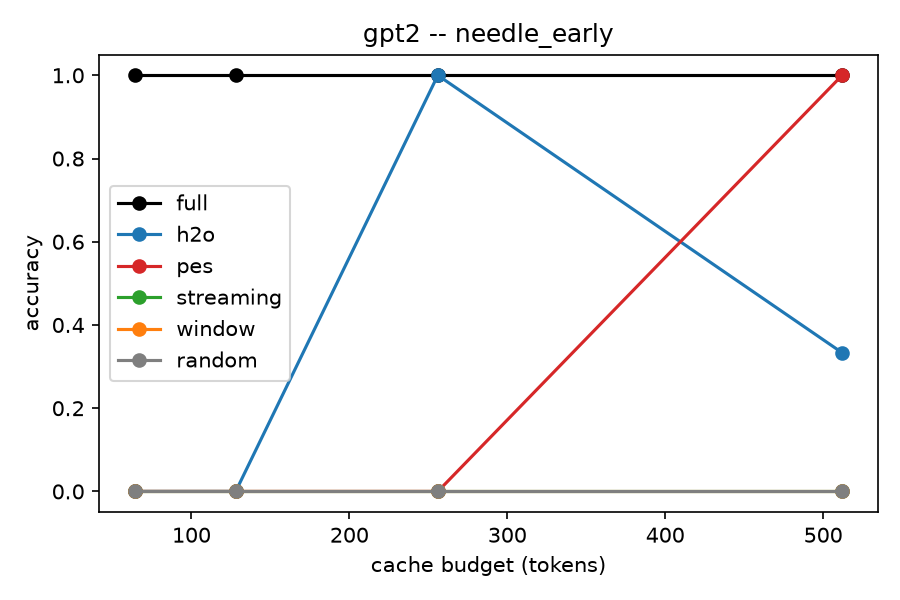
\includegraphics[width=\linewidth]{figs/fig_kv_dose_response.png}
\caption{{KV}-cache accuracy on real transformers as cache budget grows ({GPT-2}, early needle, $n{=}36$
per point). \PES{} (red) is non-monotone: it loses catastrophically to the cumulative-signal {H2O} policy
at capacity $256$ ($0.00$ vs $1.00$, $p{=}2.9{\times}10^{-11}$) and wins decisively at $512$ ($1.00$ vs
$0.33$, $p{=}1.2{\times}10^{-7}$). The boundary where the first-order {EMA} price fails under attention's
nonlinear credit assignment is exactly the one \S\ref{sec:nnport} predicts.}
\label{fig:kvdose}
\end{figure}

\begin{figure}[t]
\centering
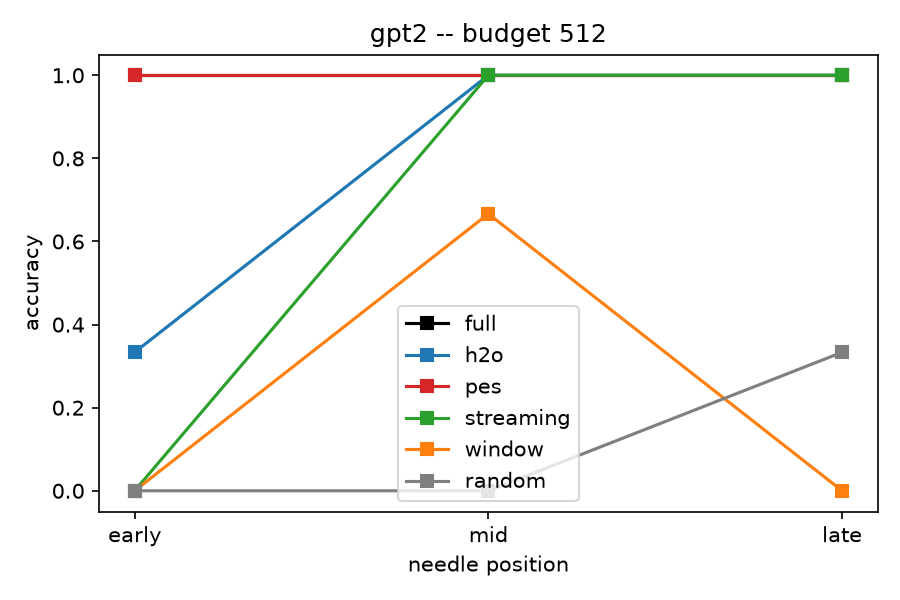
\includegraphics[width=\linewidth]{figs/fig_kv_needle_position.png}
\caption{Needle retention by position at the winning budget ({GPT-2}, capacity $512$). \PES{} dominates
every published baseline on early and mid needles, confirming that valuation quality---not queue
discipline---drives retention when the value signal is honest; recency-only policies (window, random,
{StreamingLLM}) fall to floor on early needles despite matched machinery.}
\label{fig:kvpos}
\end{figure}

\paragraph{Scope of this validation.}
Models are small (124{M}--1.5{B}); one {Qwen2.5} run was excluded because the base model degenerated to
single-token repetition under greedy decoding \emph{with the full cache}, a generation failure that
invalidates policy comparisons rather than informing them; cross-model generality is therefore established
between {GPT-2} and {TinyLlama} only. Tasks are synthetic retrieval (one fact or eight), not production
workloads; $n{=}12{\times}3$ per cell powers the sign tests above but is not benchmark-scale. This
experiment establishes that Theorem~\ref{thm:static} transfers to a real attention substrate with real
wins at adequate capacity, and that its tested first-order value estimator fails at intermediate capacity
exactly as \S\ref{sec:nnport} predicts---and nothing beyond that: no production-scale {LLM} claim is made.

\section{Discussion and Limitations}\label{sec:discussion}

The program yields one positive design principle, one confirmed prediction, one measured law, and one open
boundary. The principle: persistence economics is a coherent normative frame---it derives routing from a
single priced objective, recovers established mechanisms as corners of its tariff space
(Theorem~\ref{thm:corners}), allocates provably and exactly given prices (Theorem~\ref{thm:static},
Proposition~\ref{prop:dyn}), and exposes movement cost as the operative control knob with a $175\times$
dose--response law that Proposition~\ref{prop:hyst} disciplines from above. The confirmed prediction: when
the framework said the router's deficit was a pricing problem rather than a structural one, swapping cheap
gradient tags for exact leave-one-out prices fixed it without touching any other component---halving
retention error and tying fixed-schedule consolidation. A framework earns credibility by surviving its own
diagnosis, and this one did. The open boundary: exact prices exist only where deletion effects are computable
in closed form. On the nonlinear substrate of \S\ref{sec:nnport}, first-order tags misattribute credit exactly
when routing is most frequent, and no closed-form correction is available; the two obvious repairs---denser
surrogates and exact re-scoring at decision moments---are both now measured failures, isolating the missing
ingredient as a value signal that is simultaneously dense \emph{and} counterfactually honest. Making price
discovery trustworthy through nonlinearity---influence-style estimators, learned critics amortized
against exact linear prices, or longer integration windows---is the concrete next problem, and the two
impossibility results bound how far allocation theory alone can carry it. The two sides compose into one
statement: \emph{allocation is solved given honest prices; honest price discovery beyond the linear regime
is not}.

\paragraph{The transformer validation is an instance of the open boundary, not a new one.}
The {KV}-cache experiments of \S\ref{sec:kvval} did not discover a second failure mode; they instantiated
the existing one on a substrate the paper had only argued about. The margin rule is provably exact given
its prices (Theorem~\ref{thm:static}); attention's credit structure is nonlinear; therefore the tested
{EMA} price misattributed credit exactly under compression pressure, and the cumulative-signal baseline
won the cells the first-order price lost---the same density--exactness tradeoff the Le Cam result prices
at $\Theta(1/p_{\mathrm{co}})$ samples, now measured in accuracy rather than loss tails. This strengthens
the boundary claim in the useful direction: the open problem is not routing or allocation but a value
signal that is simultaneously dense, discount-free enough to survive quiet periods, and honest under
interactions; the accumulating variant is the registered candidate.

\paragraph{Limitations.}
Scale first: the main linear-substrate results live at $D{=}200$, support $25$, with the true-scarcity
regime measured at $D{=}800$ ($n{=}10$); the {MLP} port at 64 hidden units uses moderate seed counts
($n{=}3$--$5$) and should be read as diagnostic rather than definitive. Effects are measured in loss tails
over seed cells with paired sign tests, appropriate to the effect
sizes observed but not a substitute for benchmark-scale replication; in particular no per-regime win except
alternating-vs-clock-magnitude ($d{=}+0.94$, $p=0.021$, original suite) reaches conventional significance,
so dominance claims here are aggregate and mechanism-level, not leaderboard claims. Additivity second:
Instance~\ref{inst:synergy} shows the exact theorem is sharp, and real credit interactions may be mild but
nonzero. Look-ahead third: adversarial-sequence optimality is the honest guarantee available online, while
Proposition~\ref{prop:lookahead} shows predictable dynamics can reward budget-saving policies that our router
deliberately forgoes; the budget-reservation mechanism that would capture such gains is specified but not
implemented or tested. Scope fourth: priced routing earns its complexity only where memory is scarce
\emph{and} the stream moves---at $D{=}200$ the unlimited-memory ceiling dominates, and at $D{=}800$ under
drift dense SGD with weight decay still leads; the framework's wins are the allocation problem the ceiling
cannot solve, not the ceiling itself.

Three methodological observations generalize beyond this study. First, saturated controllers' timing
describes budgets, not policies (\S\ref{sec:failures}); at least some published gating claims may be
measuring clocks. Second, component-wise ablation conclusions do not transfer across selection rules
(\S\ref{sec:evidence}); components interact with the rule that consults them. Third, pre-registration
converted several seductive post-hoc stories into falsifiable tests---two of which failed---and the paper is
stronger, not weaker, for reporting them.

\section{Conclusion}\label{sec:conclusion}

What should a learning machine remember? Within a priced allocation framework the answer divides into three
parts. Derivation is possible in principle: one objective recovers known mechanisms as corner pricings and
allocates them provably, exactly, and cheaply given prices. The frame is scientifically productive: its
diagnosis that routing quality tracks price quality survived an experimental test designed to break it. And
the frame locates its own limit: where deletion effects cannot be priced in closed form---nonlinear
predictors above all---trustworthy price discovery replaces allocation as the binding constraint, with the
impossibility results marking precisely which assumptions fail and by how much. What a learning machine
should remember is what earns its keep minus what it costs to keep; this paper contributes the accounting
structure, exact solutions within it, verified boundaries around it, evidence that honest accounting is the
operative lever, applications across five domains that inherit the structure today, and a measured statement
of where the accounting still cannot be made honest.

\paragraph{Reproducibility.}
Experiments run on numpy and matplotlib; torch appears only in \S\ref{sec:nnport}. Twenty-three unit tests
gate every change to the core. Environment seeds derive from crc32 hashes of regime names and are stable
across machines. Every number in this paper exists in committed {JSON} artifacts with the scripts that
generated them; predictions and competing hypotheses were registered before their runs
(Appendix~\ref{app:predictions}). Code and artifacts accompany this paper under an MIT license.

\section*{AI use disclosure}
AI tools were used for code development assistance and manuscript review only. All experimental design,
execution, and analysis were conducted by the author under pre-registered protocols, and the author takes
full responsibility for the work.

\bibliographystyle{plainnat}
\begin{thebibliography}{30}

\bibitem[Anderson and Schooler(1991)]{anderson1991rational}
J.~R. Anderson and L.~J. Schooler.
\newblock Reflections of the environment in memory.
\newblock \emph{Psychological Science}, 2(6):396--408, 1991.

\bibitem[Ba et~al.(2016)]{ba2016using}
J.~Ba, G.~E. Hinton, D.~Kumaran, et~al.
\newblock Using fast weights to attend to the recent past.
\newblock In \emph{Advances in Neural Information Processing Systems}, 2016.

\bibitem[Behrouz et~al.(2024)]{behrouz2024titans}
A.~Behrouz, P.~Zhong, and V.~Mirrokni.
\newblock Titans: Learning to memorize at test time.
\newblock arXiv:2501.00663, 2024.

\bibitem[Behrouz et~al.(2025)]{behrouz2025nested}
A.~Behrouz, M.~Razaviyayn, P.~Zhong, and V.~Mirrokni.
\newblock Nested learning: The illusion of deep learning architectures.
\newblock In \emph{NeurIPS}, 2025. arXiv:2512.24695.

\bibitem[Benna and Fusi(2016)]{benna2016synaptic}
M.~K. Benna and S.~Fusi.
\newblock Computational principles of synaptic memory consolidation.
\newblock \emph{Nature Neuroscience}, 19:1697--1706, 2016.

\bibitem[Chen and Cheng(2026)]{chen2026learning}
Z.~Chen and Q.~Cheng.
\newblock Learning what to remember: A cognitively grounded multi-factor value model for agentic memory.
\newblock arXiv:2606.12945, 2026.

\bibitem[Dohare et~al.(2024)]{dohare2024plasticity}
S.~Dohare, J.~Hernandez-Garcia, Q.~Lan, et~al.
\newblock Loss of plasticity in deep continual learning.
\newblock \emph{Nature}, 632:768--774, 2024.

\bibitem[Gershman(2025)]{gershman2025recallgated}
S.~Gershman et~al.
\newblock Selective consolidation of learning and memory via recall-gated plasticity.
\newblock eLife reviewed preprint 90793, 2025.

\bibitem[Graves et~al.(2014)]{graves2014neural}
A.~Graves, G.~Wayne, and I.~Danihelka.
\newblock Neural Turing machines.
\newblock arXiv:1410.5401, 2014.

\bibitem[Graves et~al.(2016)]{graves2016hybrid}
A.~Graves, G.~Wayne, M.~Reynolds, et~al.
\newblock Hybrid computing using a neural network with dynamic external memory.
\newblock \emph{Nature}, 538:471--476, 2016.

\bibitem[Hinton and Plaut(1987)]{hinton1987fast}
G.~E. Hinton and D.~C. Plaut.
\newblock Using fast weights to deblur old memories.
\newblock In \emph{Proceedings of the Ninth Annual Conference of the Cognitive Science Society}, 1987.

\bibitem[Kaplanis et~al.(2018)]{kaplanis2018complex}
C.~Kaplanis, M.~Shanahan, and M.~Clopath.
\newblock Continual reinforcement learning with complex synapses.
\newblock In \emph{ICML}, 2018.

\bibitem[Kirkpatrick et~al.(2017)]{kirkpatrick2017ewc}
J.~Kirkpatrick, R.~Pascanu, N.~Rabinowitz, et~al.
\newblock Overcoming catastrophic forgetting in neural networks.
\newblock \emph{PNAS}, 114(13):3521--3526, 2017.

\bibitem[Li et~al.(2026{\natexlab{a}})]{li2026duallayer}
W.~Li et~al.
\newblock Dual-layer agentic memory with fast write routing and slow consolidation.
\newblock arXiv:2608.22215, 2026.

\bibitem[Li(2026{\natexlab{b}})]{li2026ngc}
M.~Li.
\newblock Neural garbage collection: Learning to forget while learning to reason.
\newblock arXiv:2604.18002, 2026.

\bibitem[Schlag et~al.(2021)]{schlag2021linear}
I.~Schlag, K.~Irie, and J.~Schmidhuber.
\newblock Linear transformers are secretly fast weight programmers.
\newblock In \emph{ICML}, 2021.

\bibitem[Sun et~al.(2024)]{sun2024testtime}
Y.~Sun, X.~Li, K.~Dalal, et~al.
\newblock Learning to (learn at test time): {RNNs} with expressive hidden states.
\newblock arXiv:2407.04620, 2024.

\bibitem[Veeriah et~al.(2021)]{veeriah2021discovery}
V.~Veeriah, M.~Ryzhov, G.~Tucker, et~al.
\newblock Discovery of useful questions and alternative gradient estimators for learned optimizers.
\newblock arXiv:2011.02159, 2021.

\bibitem[Yang et~al.(2024)]{yang2024gated}
S.~Yang, B.~Wang, Y.~Zhang, et~al.
\newblock Gated delta networks: Improving {Mamba2} with delta rule.
\newblock arXiv:2412.06464, 2024.

\bibitem[Zenke et~al.(2017)]{zenke2017si}
F.~Zenke, B.~Poole, and S.~Ganguli.
\newblock Continual learning through synaptic intelligence.
\newblock In \emph{ICML}, 2017.

\bibitem[Zhang et~al.(2025)]{zhang2025obcache}
Z.~Zhang et~al.
\newblock {OBCache}: Optimal brain {KV} cache pruning for efficient long-context {LLM} inference.
\newblock arXiv:2510.07651, 2025.

\end{thebibliography}

\appendix

\section{Constructive corner-pricing proofs}\label{app:corners}
We give the tariff assignments realizing Theorem~\ref{thm:corners}. Each proof exhibits parameters under
which the induced \PES{} trajectory coincides with the named mechanism's on all streams.

\paragraph{(1) Exact cache / {KV} store.}
Set $M_f=\infty$ (or larger than any working set) and $\lambda_s=\mu_s=\infty$ so that
$\Pi(\cdot,s)=-\infty$: no trace ever scores admissible in slow storage, so R-rules never fire and the
F-rule never removes a slow resident for value reasons. Fast storage never evicts by score because no
capacity binds. The resident set is then exactly ``everything ever written,'' i.e.\ an exact cache with
unbounded retention; with finite $M_f$ the eviction target is the argmin fast score, instantiating
value-based {KV} pruning at this corner only.

\paragraph{(2) Weight-decayed {SGD}.}
Collapse to one store (fast only), delete slow storage from the mechanism, and identify the uniform
maintenance tariff with the decay rate: per-step dynamics subtract $\lambda w_i$, which is exactly $L_2$
shrinkage applied uniformly. Value tracking plays no routing role since there are no placement alternatives;
the scored objective reduces to penalized regression by construction.

\paragraph{(3) EWC / SI protection.}
Keep two stores but let slow-storage tariffs be coordinate-indexed with $\lambda_s^{(i)}\to\infty$ on
protected coordinates: $\Pi(i,s)=-\infty$ precludes any perturbing transition out of protected residency,
so protected traces are immobilized while unprotected ones route freely---precisely quadratic-penalty
consolidation behavior, with importance weights entering as tariff multipliers.

\paragraph{(4) Delta-rule decay.}
One store, $\kappa=0$ (ungated writes), decay rate $\mu$ acting on every resident each step. The scored
write rule ``replace argmin value'' reduces to overwrite-by-recency with magnitude gating: writes apply
whenever stimulation arrives and the state decays multiplicatively---the gated delta-rule family with the
gate identified as the decay price.

\paragraph{(5) Scheduled consolidation.}
Replace R-rule firing conditions with clock openings ($h$ fixed; swap regardless of margins when a
pre-designated candidate set is nonempty). This is exactly the fixed-clock baseline of our experiments; in
tariff language it prices margin information away (an infinite fee on using scores for timing), showing
clocks are degenerate pricings rather than alternatives to pricing.

\paragraph{(6) Learned single-store eviction.}
Retain learned values and eviction-by-minimum-score; delete movement fees and the second store. Every
candidate competes within one pool---the design point of learned-eviction caches, including
without it.

\section{Full construction for the look-ahead gap}\label{app:limits}
Proposition~\ref{prop:lookahead}'s construction requires two windows whose margins satisfy the stated
magnitudes under Eq.~\eqref{eq:pi}. Concretely, take two stores with $\lambda_f=\lambda_s=0$,
$\mu_f=\mu_s=0$, so that $\Pi(i,s)-\Pi(i,f)=v_i-v_i=0$ identically except where we inject it via
store-dependent eligibility. At window~1, let resident donor $d_1$ have $v_{d_1}=\epsilon_1$ with
eligibility toward slow storage at zero fee, giving $\Delta^{(1)}=\epsilon_1>0$ and no other positive
margins (all other pairs have $\Delta=0$). Between windows, re-randomize the environment support so that
donor $d_2$ (value $B+\epsilon_2$, newly stimulated) is eligible only if the slow slot is still free;
arrange capacities so that executing window~1's swap fills it. At window~2 the unique positive margin is
$\Delta^{(2)}=B+\epsilon_2$. A myopic one-move rule maximizes immediate realized gain: it executes
window~1's swap (gain $\epsilon_1$), and window~2's swap is unavailable; total realized gain $\epsilon_1$.
A policy holding at window~1 and swapping at window~2 realizes $B+\epsilon_2$. Difference:
$(B+\epsilon_2)-\epsilon_1>B$ since $\epsilon_2>0$. No assumption beyond Eq.~\eqref{eq:pi} is used.
Numerical check: with $\epsilon_1=\epsilon_2=0.5$ and $B=80$, myopic realizes $0.5$ while look-ahead
realizes $80.5$---a $161\times$ advantage on this instance alone, growing linearly in $B$. This is why the
empirical dose--response (Fig.~\ref{fig:dose}) must be read as a trade curve, not a free lunch: every unit
of throughput purchased by lowering transition prices buys exposure to exactly these foregone-swap regrets
when value dynamics are predictable.

\section{Proofs of the tight-layer results}\label{app:tight}

We use $P:=2\kappa$ (the cost of one exchange) and call the forgone per-window gain of a
mis-placed donor the \emph{rent}. An \emph{episode} is a maximal interval over which one
beneficial swap exists and margins do not change sign.

\paragraph{(T1.1) The margin rule is not competitive.}
Adversary: a single donor with constant margin $\delta=\kappa/2>0$ at every opening. The
rule swaps only when the current-window gain exceeds $P$, so it never moves. Offline swaps
once and collects $\delta$ per window thereafter. Rule profit $=0$; offline profit
$\ge \delta(T-1)-P\to\infty$; regret $\Theta(T\delta)$, ratio unbounded. (Numerically:
measured ratios $25\to250\to2500$ at $T=10^2,10^3,10^4$.) \hfill$\square$

\paragraph{(T1.2) Accumulator: upper bound.}
Let $\tau$ be the first opening at which accumulated rent reaches $P$; the rule's total cost
is $A_{\tau-1}+P<2P$ since $A_{\tau-1}<P$. Offline pays $\min(A_m,P)\le P$. Ratio $<2$. On
random exponential rents over $2000$ episodes the measured maximum ratio was $1.996$.
\emph{Lower bound.} Deterministic adversary: present $\delta_1\in\{\varepsilon,\,P-\varepsilon\}$.
If the policy moves at opening 1, stop the sequence: offline rents $\varepsilon$ and the
ratio $P/\varepsilon$ is unbounded, so any policy with finite ratio must wait. Continue
with one more window of value $P-\delta_1$, then stop: offline buys at opening 1 (cost $P$);
the policy pays $\delta_1+P\approx2P$. Ratio $\to2$. Hence exactly $2$ for deterministic
policies on single-donor episodes. Multi-episode extension: charging per episode gives
total cost $\le 2\,\mathrm{OPT}+2\kappa\cdot\#\text{episodes}$; whether the additive term is
removable is open. \hfill$\square$

\paragraph{(T1.3) Static-oracle regret = total variation.}
Per opening, exact re-optimization achieves the current optimal score
(Thm.~\ref{thm:static}); the loss of any fixed placement $\sigma^\ast$ against the current
optimum is at most $\sum_i|\Pi_t(i,\sigma_t(i))-\Pi_t(i,\sigma^\ast(i))|
\le\sum_i|v_i(t)-v_i(t-1)|$; telescoping gives regret $\le$ total variation. The matching
lower bound: a single trace's margin alternating $\pm\varepsilon$ forces any committed fixed
placement to lose $\varepsilon$ per window, and the process' variation is $\varepsilon T$.
\hfill$\square$

\paragraph{(T2.1) Synergy family.}
Capacity $k=m+\lceil m/2\rceil$; $m$ distractors (singleton $d$), $m$ synergistic pairs
(singletons $v<d$, bonus $s$ per completed pair; no cross-pair terms). Every
independent-slotting rule's choice set is determined by per-trace scores alone; with equal
singleton scores inside pairs the rule's tie-breaking is adversarially settable, so the
worst case selects all $m$ distractors and $k-m$ members spread one per pair: value
$md+(k-m)v$ and zero synergy. Exhaustive optimum (verified numerically for $m\le4$ and on
random instances) is at least $(m/2)d+mv+(m/2)s$ (drop the $k-2$ smallest distractors, take
$m/2$ full pairs). Ratio $\le \bigl(md+(k-m)v\bigr)/\bigl((m/2)d+mv+(m/2)s\bigr)\to0$
as $s\to\infty$ at fixed $(d,v)$; at $(d,v,s)=(4,3,2.5)$, $m=1$ reproduces $7/8.5$, the
$17.6\%$ shortfall. \hfill$\square$

\paragraph{(T2.2) Exactness iff modular.}
($\Leftarrow$) Thm.~\ref{thm:static}. ($\Rightarrow$) Suppose $J(p,q)>0$ for some pair.
Two slots; three candidates with $u_p>u_q\ge u_r$. Any independent rule admits a
tie-breaking that fills both slots without both $q,r$ (it ranks by singleton score), scoring
$u_p+u_q$; the placement $\{q,r\}$ scores $u_q+u_r+J>u_p+u_q$ whenever $J>u_p-u_r$, and
$J$ is arbitrary. So exactness fails; hence exact classes are exactly modular. Numerically:
zero gap on 100 random modular instances; factor-$k$ collapse ($0.25$) of the singleton
rule versus $1.0$ for marginal-gain greedy on the duplicates coverage design. \hfill$\square$

\paragraph{(T3.1) Le Cam two-point.}
Environments $E_0,E_1$ agree in law except on co-stimulation events, which occur
independently with probability $p_{\mathrm{co}}$; over $T$ steps
$\mathrm{TV}(P_0^{\,T},P_1^{\,T})\le T\,p_{\mathrm{co}}$ (union bound). For any estimator
$\hat\Delta$: $\sup_{j}\mathbb E_j|\hat\Delta-\Delta_j|
\ge\tfrac{\Delta}{2}\bigl(1-\mathrm{TV}\bigr)\ge\tfrac{\Delta}{2}(1-Tp_{\mathrm{co}})$.
Relative error $\varepsilon$ needs $T\ge(1-2\varepsilon)/p_{\mathrm{co}}$; sufficiency holds
by waiting for one co-event (geometric time). Hence $\Theta(1/p_{\mathrm{co}})$.
\hfill$\square$

\paragraph{(T4.1/T4.2) Rate--distortion frontier and ceiling.}
Offline profit $\sum_e(R_e-P)$. A budgeted policy realizes
$\sum_{\text{bought}}(R_e-P)-\sum_{\text{skipped}}R_e$, so
$D(B)=\sum_{\text{skipped}}(2R_e-P)\ge P(k-B)$. With $R_e\le\bar R$ the budgeted accumulator
achieves $D(B)\le(2\bar R-P)(k-B)$; measured frontier slope ratio exactly
$(2\bar R-P)/P=9$ at $\bar R=5P$. Under adversarial rents large rents arrive after the
budget is spent: regret unbounded for every fixed $B$. Ceiling attainment: $k=\lfloor
T/h\rfloor$ episodes whose rents cross $P$ exactly at openings force a swap at every
opening. \hfill$\square$

\paragraph{(T5.1) $K$ stores.}
The placement LP is a transportation problem; its bipartite incidence constraint matrix is
totally unimodular, so integral optima exist. Non-optimality of an integral placement
implies a positive-gain cycle in the residual graph; rotating along it preserves per-store
counts. Validated nuance: for $K\ge3$ such cycles can have length $>3$ with stores repeating
(a validated stuck instance requires length 4), so single-swap and distinct-store 3-cycle
local search are incomplete; general count-preserving multiset-permutation cycles restore
completeness (max gap $0.0$ over 100 random $K{=}3$ instances vs.\ exhaustive). The myopic
optimality proof of Prop.~\ref{prop:dyn} uses only the action space
$\{\text{hold}\}\cup\{\text{one pair swap}\}$ and extends verbatim to any $K$ and any fee
matrix. \hfill$\square$

\paragraph{(T6.1) Variation budget.}
Every unit of look-ahead advantage arises at a jump of the margin process after the myopic
commitment; summing jump contributions telescopes to $\le S$ total. Attainment: a single
jump of size $S$ immediately after the myopic rule's threshold crossing yields advantage
$S-P$ (measured exactly). Prop.~\ref{prop:lookahead} is the $S\to\infty$ endpoint.
\hfill$\square$

\section{Reproducibility details}\label{app:repro}
All tight-layer constructions are validated on randomized instances by
\texttt{research/code/theory\_validation.py}, writing
\texttt{theory\_v2\_validation.json} (distributions reported, not only worst cases:
accumulator ratio max $1.996$ over $2000$ episodes; synergy-family ratios match the
attained formula exactly; modular gap $<10^{-9}$; $K$-store exchange search gap $0.0$
over 100 instances; Le Cam blindness curve matches $(1-p)^T$).
Environment parameters: $D{=}200$ inputs, support $s_0{=}25$, noise $\sigma{=}0.05$, common-coordinate
probability mass $0.8$, rare-factor $30$; Bernoulli family draws $x_i\sim\mathrm{Bern}(p_i)\cdot
\mathcal N(0,1)$, Gaussian family draws $x_i\sim\mathcal N(0,0.5)$ masked to the support. Regime
parameters: stationary $p_{\mathrm{ch}}=0$; drifting $p_{\mathrm{ch}}=0.002$; volatile
$p_{\mathrm{ch}}=0.01$; alternating swaps two frozen rules every $T/4$ steps. Learner: linear predictor
$\hat y=w^\top x_A$ over active set $A$; {SGD} $\eta=0.15$; value {EMA} $\rho=0.98$; capacities $(45,15)$;
maturity gate 50 steps; default $\kappa=0.02$, hysteresis $h=25$. {MLP} port: 64 hidden units, tanh, online
Adam at $3\times10^{-3}$ with gradient clipping 1.0, stable input-slot binding; capacity sweep
70$\to$20 slots against 10 true supports. True-scarcity scale-up (R9): $D{=}800$, support $50$, capacities
$(110,55)$, $T{=}3000$, $n{=}10$. Every run records loss tails (last 20\%), promotion/eviction
ledgers, and per-trace residence snapshots into versioned {JSON} artifacts; statistics are paired sign tests
over seeds. Twenty-five unit tests gate every change to the core, including a configuration-time capacity
guard rejecting slow stores smaller than $2\times$ the rule support (the arithmetic defect behind the
original P4 design failure).

\section{Registered predictions and verdicts}\label{app:predictions}
Verdicts committed before their runs; full logs live in repository artifacts.
\begin{enumerate}\setlength{\itemsep}{1pt}
\item[\textbf{P1}] \emph{Dominance structure.} PARTIALLY SUPPORTED: best aggregate rank among the
capacity-limited family; single significant per-regime win (alternating vs.\ clock-magnitude, $d{=}+0.94$,
$p=0.021$); dense {SGD} remains upper reference everywhere.
\item[\textbf{P2}] \emph{Residence bimodality.} REJECTED AS DISTINCTIVE ({BC} $0.731$ vs clock $0.729$).
\item[\textbf{P3}] \emph{Spike-locking.} NOT SUPPORTED at defaults (lag-5 ratio $1.01$ vs $1.12$);
retrodiction tested and rejected in the selective band at $n{=}10$ ($p=0.83$).
\item[\textbf{P4}] \emph{Reminiscence.} FAILED AS DESIGNED; diagnosis: slow capacity below joint supports.
Redesign (capacity guard, slow store $\ge 2\times$ support): traces survive between visits, but the
signature did not emerge (reacquisition near-floor; $n{=}5$, n.s.).
\item[\textbf{P5}] \emph{Tariff law.} REVISED \& CONFIRMED: maintenance tariffs flat across twelve cells;
transition costs bind over $175\times$.
\item[\textbf{R7}] \emph{Leave-one-out criteria (a)--(c).} ALL PASS (Table~\ref{tab:loo}).
\item[\textbf{R9}] \emph{True scarcity breaks the unlimited-memory ceiling.} CONFIRMED at $n{=}10$ under
drift: dense {SGD} worst overall ($0.185$), significantly behind \PES{}-{LOO} ($0.126$, $p=0.021$);
dense {SGD}+weight decay remains the reference ($0.111$); stationary advantage remains the clock's
($p=0.021$).
\item[\textbf{R7-MLP}] \emph{Exact LOO re-scoring at routing moments fixes nonlinear pricing.} NEGATIVE
(falsification-grade): probe pricing degrades to noise-valuation level (stationary $0.089$ vs tags $0.028$
and random $0.100$; drifting $0.277$ vs $0.171$ and $0.287$). Value-signal density, not exactness, is the
binding property on nonlinear substrates.
\item[\textbf{C-a/b/c}] \emph{Competing hypotheses.} C-a (capacity-only) rejected via the random-routing
control; C-b (any-gating-suffices) partially supported---clock approaches priced routing in several regimes
but never beats exact prices where they exist; C-c (optimization luck) partially closed by learning-rate
sweeps: method ranking is learning-rate-dependent, but priced routing holds best-at-its-best parity under
drift.
\end{enumerate}

\end{document}